\documentclass[english,fleqn,allpages]{ISTE_science}[2018/07/30]


\setcounter{MaxMatrixCols}{30}
\usepackage{amsthm}
%\usepackage{OKS_ISTE}
%\CropMarksOn
\usepackage{natbib}
\renewcommand\bibsection{\section{\bibname}}
\setlength{\bibsep}{3pt} 
\makeatletter

%\newcounter{numdef}[chapter] \global\long\def\thenumdef{\thechapter.\arabic{numdef}}
% \global\long\def\NumberedDefinition#1


\newsavebox{\fminibox} \newlength{\fminilength} \newenvironment{fminipage}[1][\linewidth]{%
 \setlength{\fminilength}{#1 - 2\fboxsep - 2\fboxrule}
 \begin{lrbox}{\fminibox}
  \begin{minipage}{\fminilength}}{%
  \end{minipage}
 \end{lrbox}
 \noindent
 \fbox{\usebox{\fminibox}}}


\title{Hierarchy and co-evolution processes}
%
%\maketitle
%Rheology of non-spherical particle suspensions]%{%
%Setting Monographs and Edited Collections\\
%According to the \hermes{} Guidelines\\
%with the \oh{} Package}


%\author{%
%Roger \Name{Rousseau} (class, styles, and tools design)\\[2pt]
%Christian \Name{Scheen} (English documentation)}


%\date{%
%Version~\PackageVersion{}, \filedate{}}


\begin{document}
\raggedbottom
%\hbadness=2000 \emergencystretch=2em \lefthyphenmin=3 \righthyphenmin=3

%\frontmatter

%\maketitle
%\tableofcontents

%\raggedbottom
\mainmatter
%\setcounter{chapter}{9}
\chapter{Hierarchy and co-evolution processes}%{Juste \Name{Raimbault}}
\label{chap-struct}

\markboth{Hierarchy and co-evolution processes}{Hierarchy and co-evolution processes}


\authorname{Juste \Name{Raimbault}}{Center for Advanced Spatial Analysis, University College London}


% book subject "Centralités et hiérarchies des réseaux et des territoires"
% => specific geo of networks and territories


%%%%%%%%%%%%%%%%
\section{Introduction}


\subsection{Complexity and hierarchy}

Complex systems with emergent properties through self-organization processes are also most of the time exhibiting some kind of hierarchical structure. Although the term of hierarchy has several different definitions and uses in very different disciplines, ranging from political science \citep{crumley1987dialectical} to physics \citep{10.1371/journal.pone.0033799}, it seems to be intrinsically linked with complexity. \cite{lane2006hierarchy} classifies four frequent uses of the term hierarchy, namely (i) order hierarchy corresponding to the existence of an order relation for a set of elements, (ii) inclusion hierarchy which is a recursive inclusion of elements within each other, (iii) control hierarchy which is the ``common sense'' use of the term as ranked entities controlling other entities with lower rank, and (iv) level hierarchy which captures the multi-scale nature of complex systems as ontologically distinct levels (or scales). For the particular study of social systems, he concludes that hierarchical levels may be entangled, that upward and downward causations are both essential, and that at least three levels (micro, meso, macro) are generally needed to capture the complexity of such systems. In a more philosophical account of complexity, \cite{morin1980methode} constructs a hierarchical method of interdisciplinary knowledge, insists on the tension between dependancy and interdependency or between opening and closing (rejoining ideas from \cite{holland2012signals}), and develops an implicit hierarchy of social systems when hypothesizing the emergence of third-type societies (swarm intelligence between humans).

Different types of complexity may be related to different types of hierarchy as \cite{raimbault:halshs-02089520} proposes, and hierarchy would indeed be endogenous to theories of complexity. \cite{allen2017multiscale} develop a multiscale information theory in which the information profile across scales, or hierarchical levels, allows quantifying the complexity of a system. The complex adaptive system theory of \cite{holland2012signals} considers complex systems as systems of boundaries that filter signals, implying an inclusion and scale hierarchy between boundaries. Theories of scaling as the one synthesized by \cite{west2017scale} rely on the quantification of hierarchy in certain dimensions of systems, captured by exponents of scaling laws. Hierarchy may be endogenous to complexity, or to knowledge of the complex itself, since for example \cite{fanelli2013bibliometric} provides empirical evidence of a ``hierarchy of sciences'', in the sense of possibility to reach theoretical and methodological consensus. This corresponds in some sense to the ``ontological complexity'' of \cite{pumain2003approche}, which relies on the number of viewpoints needed to grasp a system, or the number of perspectives in an applied perspectivism framework \citep{raimbault2020relating}. Wether linked to systems themselves or to models and theories of them, hierarchy appears to be tightly linked to complexity.



\subsection{Territorial systems and hierarchy}


Urban systems, and more generally territorial systems, are particularly linked to hierarchy \citep{pumain2006hierarchy}: they indeed encompass all the meanings aforementioned (order hierarchy between settlement sizes for example, inclusion hierarchy between territorial boundaries, control hierarchy through governance structure, and more importantly level hierarchy through their multi-scalar nature). \cite{batty2006hierarchy} shows that hierarchies are inherent to urban systems, as fat tail distribution of settlement size are already produced by simple models of urban growth, and suggests also that urban design processes imply underlying overlapping hierarchies. \cite{pumain2006alternative} links hierarchical selection and hierarchical diffusion of innovation across cities to the long-term dynamics of urban systems. \cite{pumain:halshs-02303136} recalls that interactions in systems of cities are tightly linked to the emergence of urban hierarchies. Generally, scaling laws in urban systems can be considered as systematic manifestations of a hierarchical structure \citep{pumain2004scaling}, which is more complex than a simple order hierarchy, since scaling patterns vary with the definition of cities \citep{cottineau2017diverse}

Hierarchical properties can be observed on several dimensions of urban systems. For example, transportation systems are hierarchical in their structure \citep{yerra2005emergence} but also patterns of use such as transportation flows \citep{jiang2009street}. Urban hierarchies are tightly related to hierarchies of their transportation links \citep{bigotte2010integrated}, and different modes of transportation networks are concerned including the air network \citep{dang2012hierarchy}. The global distribution of multinational firms also exhibits strong hierarchical patterns \citep{godfrey1999ranking}. Governance structures are organized following both an inclusion hierarchy for administrative areas \citep{li2015administrative} but also level hierarchies for example for economic processes \citep{liao2017opening}. Territorial systems are therefore intrinsically hierarchical in their multiple dimensions, what is tightly linked to their different complexities \citep{2019arXiv190109869R}. 




\subsection{Co-evolution and hierarchy}



Hierarchy in complex systems is furthermore intrinsically linked to the concept of co-evolution. Following \cite{lane2006hierarchy}, the approach to complex adaptive systems proposed by \cite{holland2012signals} integrates levels and nested hierarchies, since it considers complex systems as ensembles of boundaries that filter signals. \cite{holland2012signals} formalizes complex adaptive systems as these structures of boundaries which form co-evolution niches for the elements and subsystems within a given boundary. The concept is slightly different from the concept of ecological niche which more generally designates a region in a parameter space quantifying the environment in which a species can live. In ecology, \cite{pires2011food} show that the emergence of mutualistic species networks imply some feeding hierarchy.

In the context of economic and geographical processes, \cite{volberda2003co} distinguish for the co-evolution of firms between a genealogical hierarchy (evolutionary processes in the biological sense) and an ecological hierarchy (co-evolutionary economic processes). \cite{liu2013exploring} suggest that air networks co-evolve with firm networks and that their hierarchies are related therethrough. \cite{raimbault2019modeling} introduces a co-evolution to study interactions between transportation networks and territories, which from an urban system viewpoint in the sense of \cite{pumain2006evolutionary} relates to urban hierarchies. \cite{levinson2007co} confirm a correspondance between urban and network hierarchies in a co-evolution model. Within the SimpopNet model for the co-evolution of cities and networks \citep{schmitt2014modelisation}, discrete hierarchical level of network links corresponding to successively improved transportation technologies are a core component of simulation rules. \cite{raimbault2020unveiling} furthermore showed that the level of initial urban hierarchy in terms of rank-size slope had significant impacts on model outcomes. Studying hierarchies in the context of co-evolution transportation networks and territories is thus a relevant entry to the underlying concepts, including complexity, hierarchy, co-evolution and territorial systems.



\subsection{Proposed approach}

\cite{pumain2006introduction} recalls in the context of social systems some remaining open methodological questions: how are hierarchies produced? How do hierarchies evolve? What discriminates between continuous and discrete hierarchical organisations? Our contribution brings new elements of answer to the first two questions above, in the particular case of co-evolution of transportation networks and territories. It situates at the intersection of the three previously given contexts, namely hierarchy in complex systems and more particularly territorial systems, seen through the prism of co-evolutive processes.

More precisely, we propose to systematically explore a macroscopic co-evolution model for cities and networks, and study its properties regarding both hierarchies of each components, in terms of final hierarchy produced but also in terms of the relations between these hierarchies. Establishing links between microscopic processes and emergent hierarchical patterns through model exploration informs on possible drivers of these macroscopic patterns. Our contribution relies on three aspects: (i) we introduce a comprehensive set of indicators tailored to the study of hierarchy in territorial systems; (ii) we systematically explore the version with a physical network of the co-evolution model introduced by \cite{raimbault2018modeling} which only studied extensively the virtual network; and (iii) we apply a novelty search algorithm to establish the feasible space of hierarchy patterns which can be produced by the model.

The rest of this chapter is organized as follows. We first describe the model used and introduce a novel set of indicators to quantify hierarchy in territorial systems. We then describe the results of a grid exploration of the co-evolution model using these indicators, both with the physical and virtual networks, and establish the feasible space of model outputs. We finally discuss the implications of these results for hierarchy within co-evolutionary processes.


%%%%%%%%%%%%%%%%
\section{Co-evolution model}

\subsection{Context}

The issue of interactions between transportation networks and territories remains an open question for which different approaches have been proposed \cite{offner1993effets,espacegeo2014effets}. \cite{raimbault2018caracterisation} has explored a co-evolution approach, in the sense that both dynamics have circular causal relationships. More precisely, \cite{raimbault2019modeling} introduces a definition of co-evolution in that particular context, based on the aforementioned co-evolution niches \citep{holland2012signals}, for which an empirical characterization method based on lagged correlations is developed \citep{raimbault2017identification}. As its application on empirical data yield various or inconclusive results, the use of simulation models is a medium to indirectly link microscopic processes with a potentially emergent co-evolution, both at the mesoscopic scale \citep{raimbault2019urban} and at the macroscopic scale \citep{raimbault2018modeling}. This latest model is the one used in this study.

\subsection{Model description}

The co-evolution model for cities and transportation networks at the macroscopic scale extends the spatial interaction model introduced by \cite{raimbault2018indirect} by adding dynamical speeds to network links. A system of cities is represented as cities as agents and network links between these. Interaction flows are determined with a spatial interaction model, and they determine city growth rates, while network links evolve according to the flow traversing them. See \cite{raimbault2018modeling} for a full mathematical description of the model. We describe below the specification and parameters used here.

More precisely, a time step of the simulation model consists in the following steps:
\begin{enumerate}
	\item cities evolve their populations following gravity interaction flows of unit weight $w_G$, as a scaling function of population with exponent $\gamma_G$, and with a distance decay parameter $d_G$;
	\item flows are assigned to network links, either (i) to the direct link between the two cities in the case of the virtual network, or (ii) through a shortest path assignment algorithm (betweenness centrality) in the case of a physical network;
	\item links evolve their speed with a thresholded self-reinforcement function of flows, with maximal time travel decrease $g_M$; a threshold for flows above which (resp. below which) speed increase (resp. decrease) determined by a flow quantile parameter $\phi^{(q)}_0$; and as a scaling relation to relative flows with exponent $\gamma_N$.
\end{enumerate}

The model can be initialized with real data or by generating a synthetic initial configuration which has its own parameters \citep{raimbault2019space}. In our case, cities are randomly distributed in space and population follow a rank-size law with parameter $\alpha_S$. For the virtual network case, all pari links are initialized with pace one, while for the physical network case a perturbed grid network is used as described in \cite{raimbault2018modeling}. We show in Fig.~\ref{fig:examples} model runs for synthetic virtual and physical networks, and for the French system of cities with railway data. We visually observe that the number of important links is smaller in the physical case as it could be expected as infrastructure is shared by neighboring flows. For the real system, the most important links emerging correspond roughly to the actual existing high-speed lines.



%%%%%%%%%%%%
\begin{figure}
	\centering
	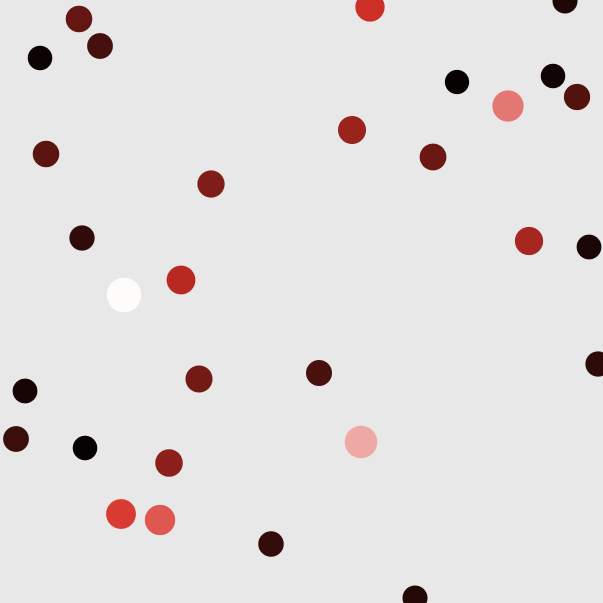
\includegraphics[width=0.48\linewidth]{figures/ex_synthvirtual_1_t0.png}
	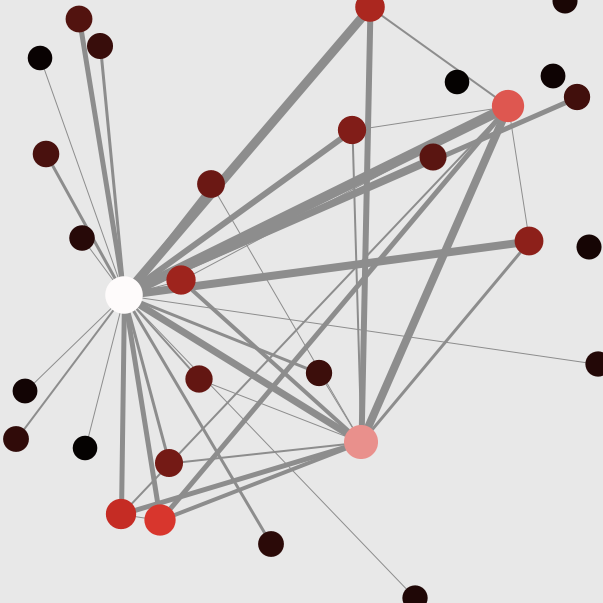
\includegraphics[width=0.48\linewidth]{figures/ex_synthvirtual_1_t30.png}\\
	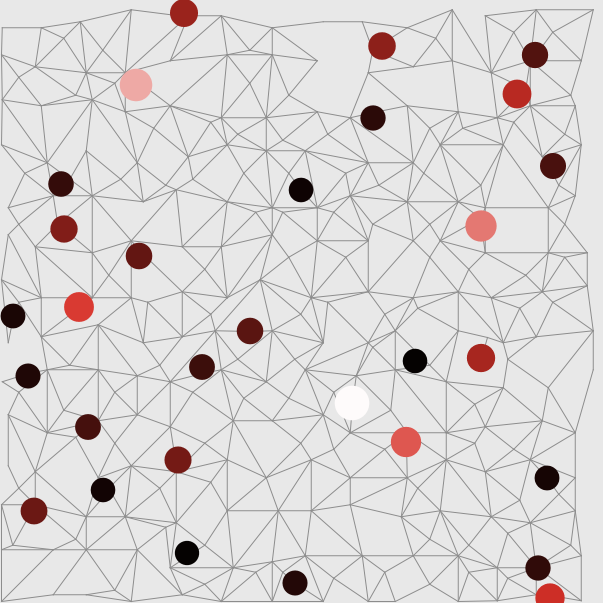
\includegraphics[width=0.48\linewidth]{figures/ex_synthphysical_1_t0.png}
	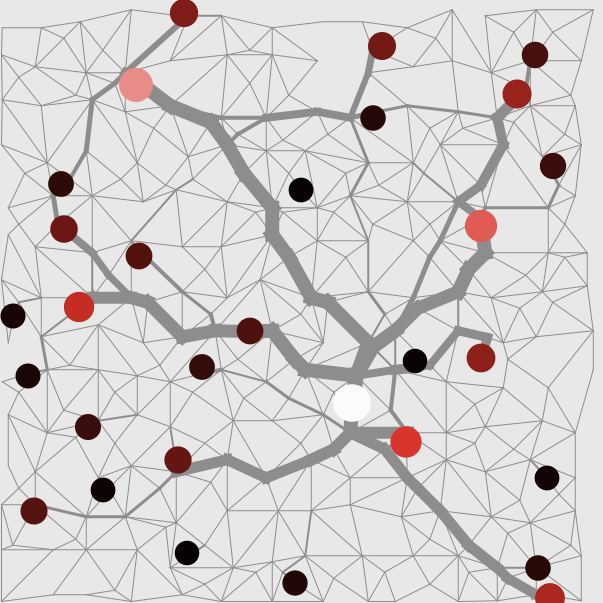
\includegraphics[width=0.48\linewidth]{figures/ex_synthphysical_1_t30.png}\\
	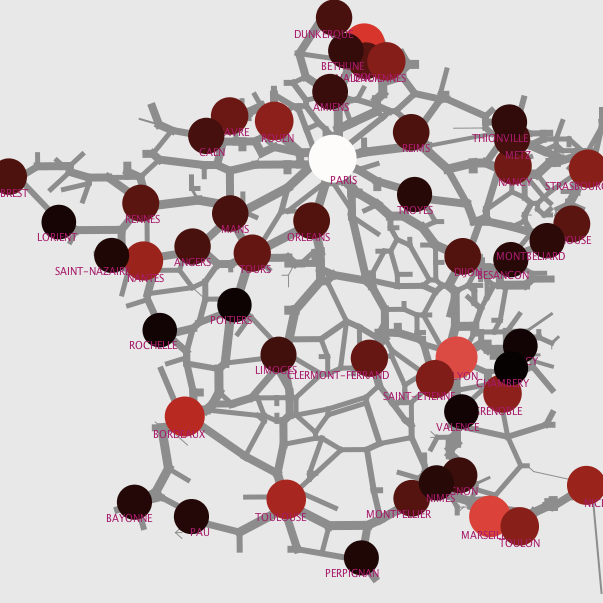
\includegraphics[width=0.48\linewidth]{figures/ex_realphysical_1975_t0.png}
	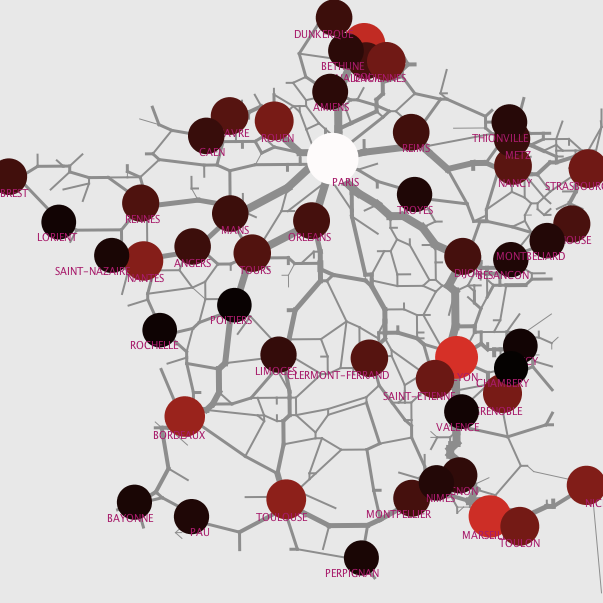
\includegraphics[width=0.48\linewidth]{figures/ex_realphysical_1975_tf.png}
	\caption{\footnotesize\textbf{Examples of different setups for the co-evolution model.} \textit{(Top row)} Synthetic system of cities with virtual network, initial configuration (left) and after $t_f=30$ time steps (right), with parameters $\alpha_S = 1$, $\phi^{(q)}_0 = 0.9$, $g_M = 0.01$, $\gamma_N=2$, $w_G=4.7e-3$, $d_G=248$, $\gamma_G=0.9$; \textit{(Middle row)} Synthetic system of cities with physical network, initial configuration (left) and after $t_f=30$ time steps (right), with parameters $\phi^{(q)}_0 = 0.7$, $g_M = 0.05$ and the same other parameters than the first configuration; \textit{(Bottom row)} French system of cities simulated between 1975 (left) and 1999 (right) with three time steps, with parameters $\phi^{(q)}_0 = 0.8$, $g_M = 0.2$, $\gamma_N=4$ and same others. City color and size give the population and link thickness the speed (rescaled at each time step).\label{fig:examples}}
\end{figure}
%%%%%%%%%%%%



\subsection{Quantifying hierarchy in systems of cities}


Indicators to understand macroscopic trajectories in simulated systems of cities have been introduced by \cite{raimbault2020unveiling}. They include some related to hierarchy but are not specifically focused on this aspect. We propose now to give a broad set of indicators to capture different dimensions of hierarchy.


\subsubsection{Static quantification of hierarchy}

The most straightforward way to quantify hierarchy is to use Zipf rank-size law in the case of population, or more generally scaling laws for other dimensions of the urban system. Let $Y_i$ the variable for which the hierarchy is estimated. Assuming $i$ is ordered in decreasing order, the Ordinary Least Square estimation of $\log \left(Y_i\right) \sim \log \left( i\right)$ gives an estimation of the rank-size slope $\alpha \left[Y\right]$ which is a proxy of hierarchy. Additional indicators to explain more accurately the size distribution include for example the primacy index. We take a generic approach to this issue of more degree of freedoms to capture the distribution and use a piecewise linear regression, implementing the algorithm of \cite{muggeo2003estimating}. Given the distribution observed empirically and the ones generated by simulation models, going beyond one breakpoint does not bring significant improvement. We consider thus the estimated slopes and breakpoint as refined indicators of the hierarchy, given as $\alpha_1 \left[Y\right]$,  $\alpha_2 \left[Y\right]$ and  $\Psi \left[Y\right]$. Finally, to quantify interactions between two aspects, a correlation between two hierarchies informs they correspond in terms of ranks, and is computed with $r_s\left[X_i,Y_i\right]$ for two variables $X_i,Y_i$ with $r_s$ an estimator of Spearman rank correlation.


\subsubsection{Dynamical indicators}

The rank correlation between initial and final distribution of a variable will measure how much an ordering hierarchy was modified, which is different from the variation of hierarchy given the variations of previous indicators such as the rank-size slope. Dynamical indicators for hierarchy regimes can furthermore be defined in several ways: dynamics of the rank correlation between two variables, time-series properties of rank-size trajectories, lagged rank correlations. Studying these extensively is out of the scope of this chapter, and we will consider differences between initial and final hierarchies to capture dynamics.


\subsubsection{Spatialized indicators}

Finally, some spatial extension of hierarchy indicators can be introduced. A spatial non-stationary version of a scaling law would write $Y_i (\vec{x}) \sim \left(\frac{X_i(\vec{x})}{X_0 (\vec{x})}\right)^{\alpha (\vec{x})}$, where $\vec{x}$ is the spatial position and assuming that samples can be defined at each point in space. In practice, a discrete version could be more relevant, for which $\vec{x}_k$ center point are defined, samples consist of points within Thiessen polygons of centers and the exponents are estimated for each center $\alpha (\vec{x}_k)$. Some heuristics should be developed to estimate such a discrete non-parametric scaling law, and also remains out of our scope here.



%%%%%%%%%%%%%%%%
\section{Results}


\subsection{Implementation}

The model is implemented in NetLogo \cite{tisue2004netlogo}, which is a good compromise between performance and interactivity, the former being necessary with a model with such a spatialized network. The model is explored using the OpenMOLE model exploration software \cite{reuillon2013openmole} to use integrated design of experiments and exploration methods, but also the seamless access its provide to high performance computing infrastructures. Source code for model, exploration scripts, result analysis, and results are available on a git repository at \url{https://github.com/JusteRaimbault/CoevolutionNwTerritories}. Large dataset for simulation results are available on the dataverse at \url{https://doi.org/10.7910/DVN/6GUKOX}.


\subsection{Hierarchy patterns}

% grid explo, compare virtual/physical
% - compare abstract network with physical (Theo Quant results) (not necessary calibration here? )

%%%%%%%%%%%%%%
\begin{figure}
\centering
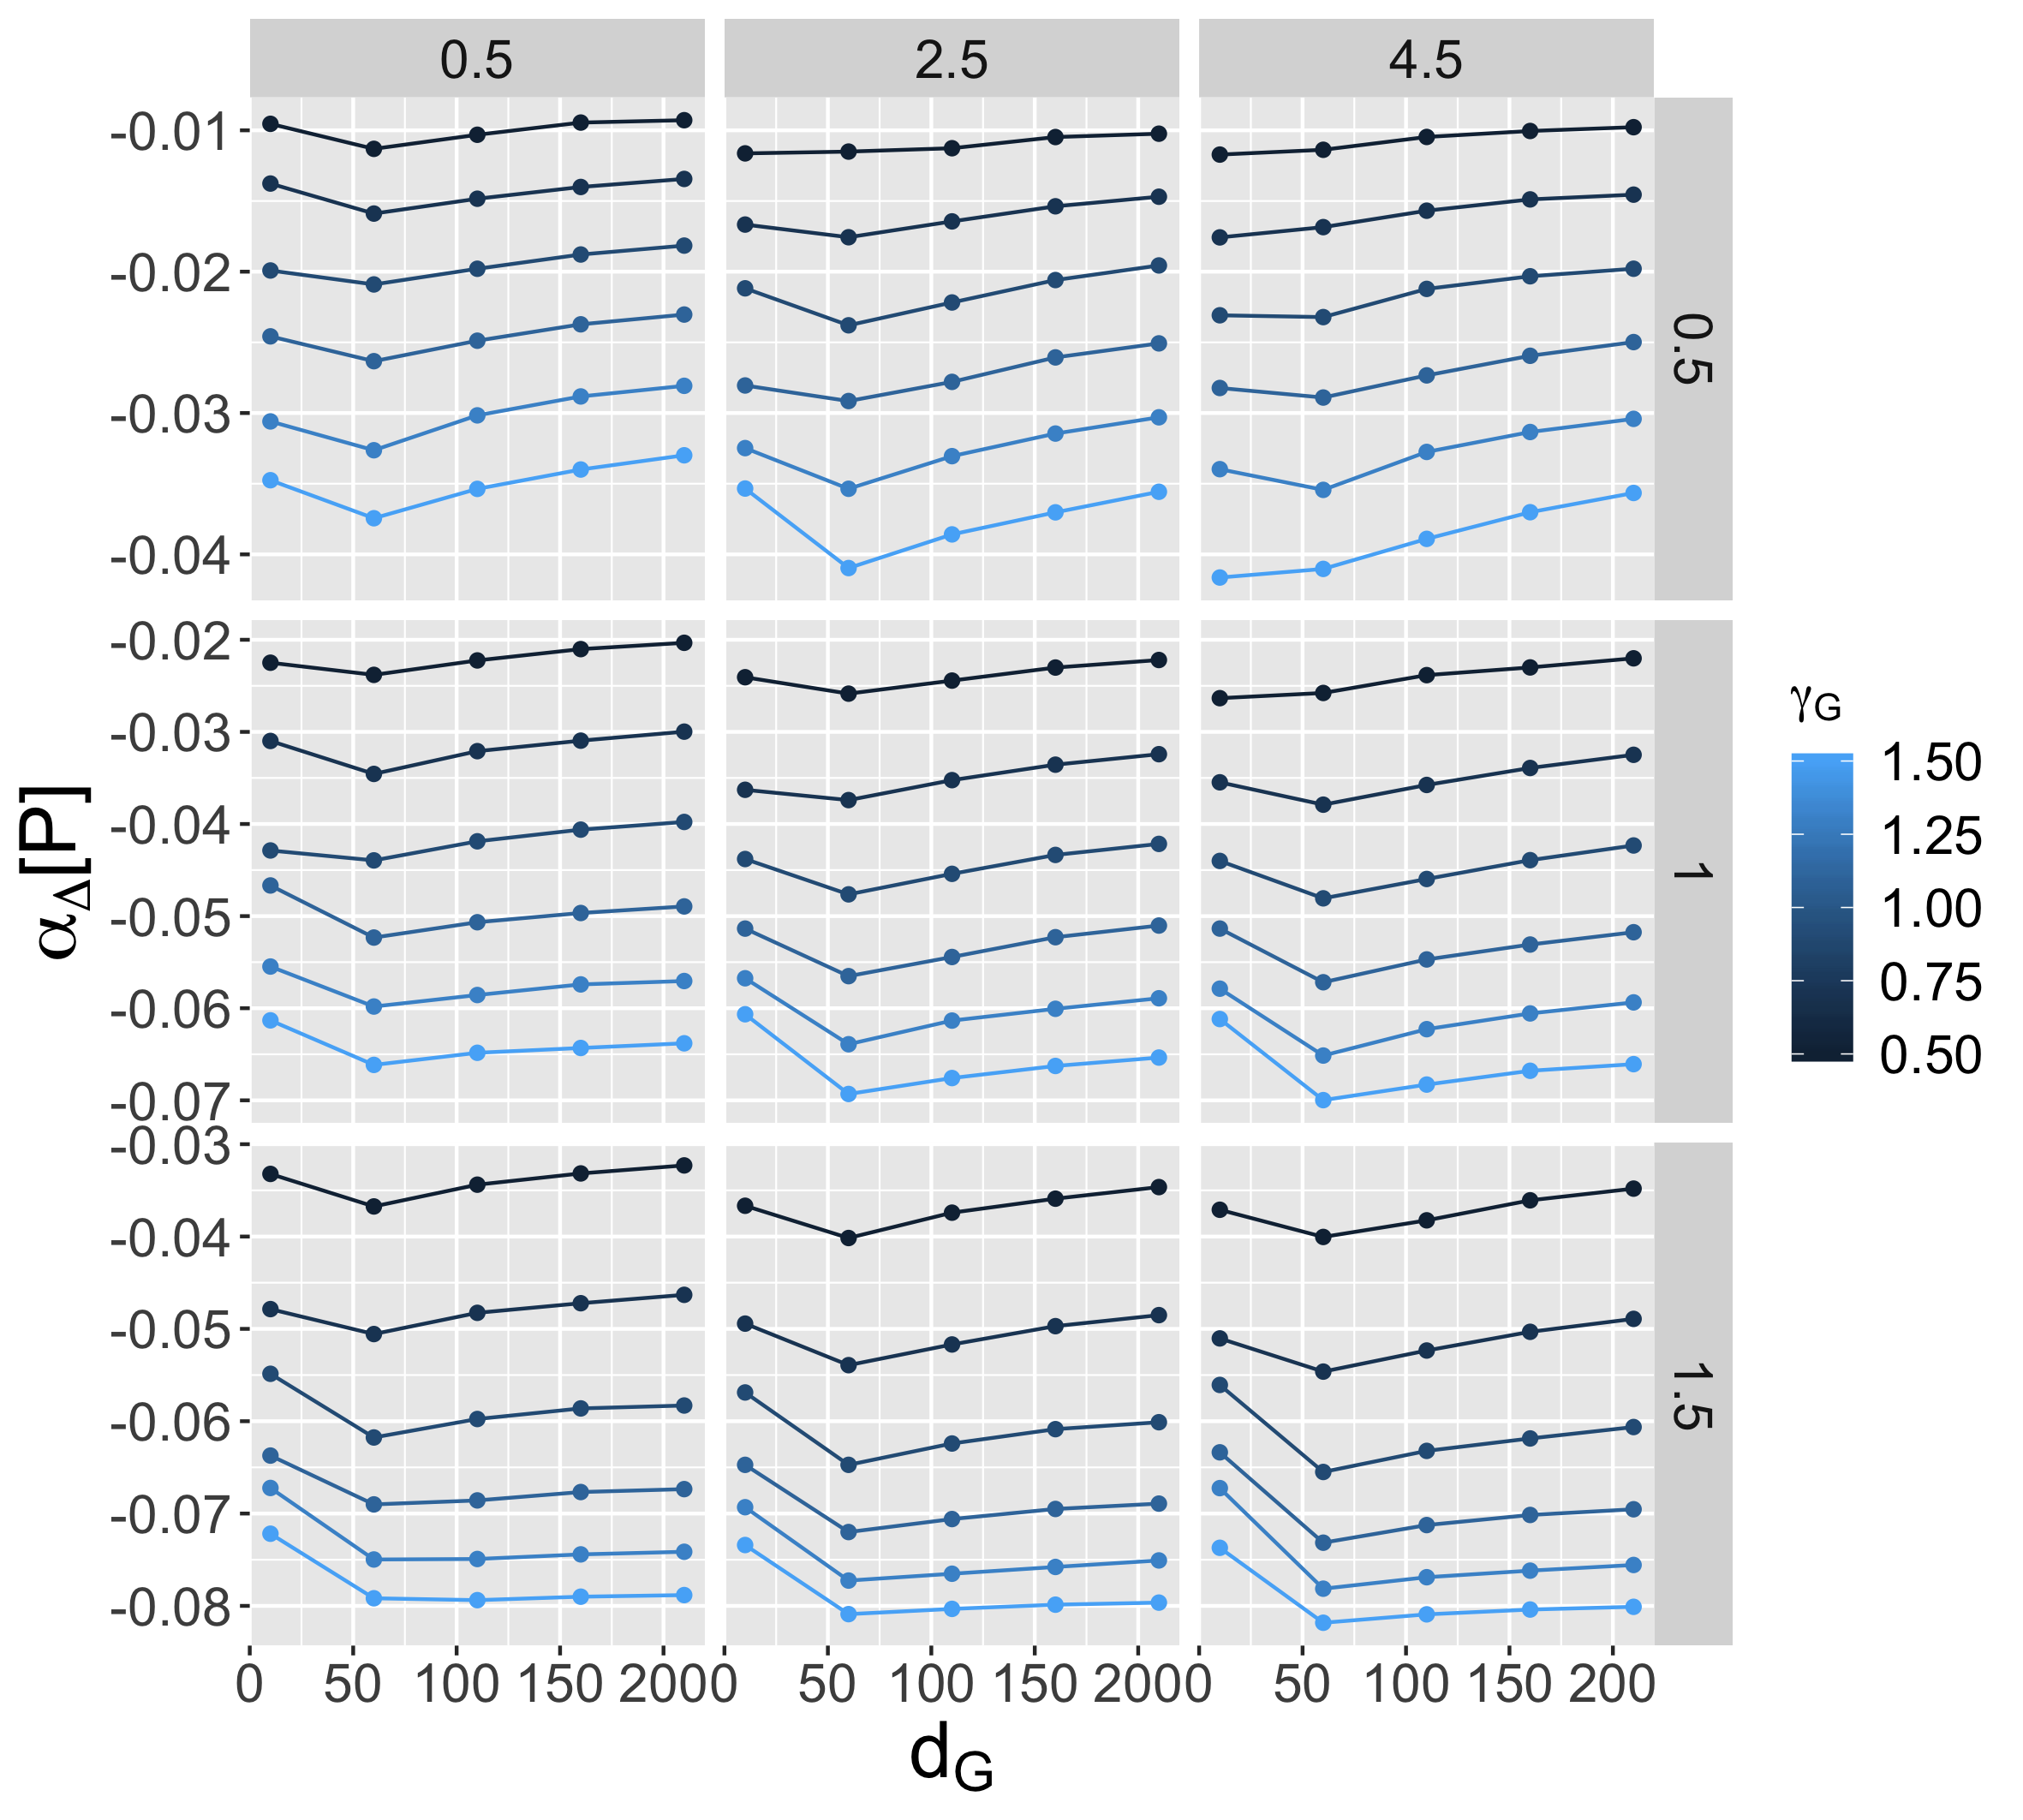
\includegraphics[width=0.48\linewidth]{figures/hierarchiesPopAlpha_nwExp1_wG0_001_xgravityDecay_colgravityGamma_facetsynthRankSize-nwThreshold.png}
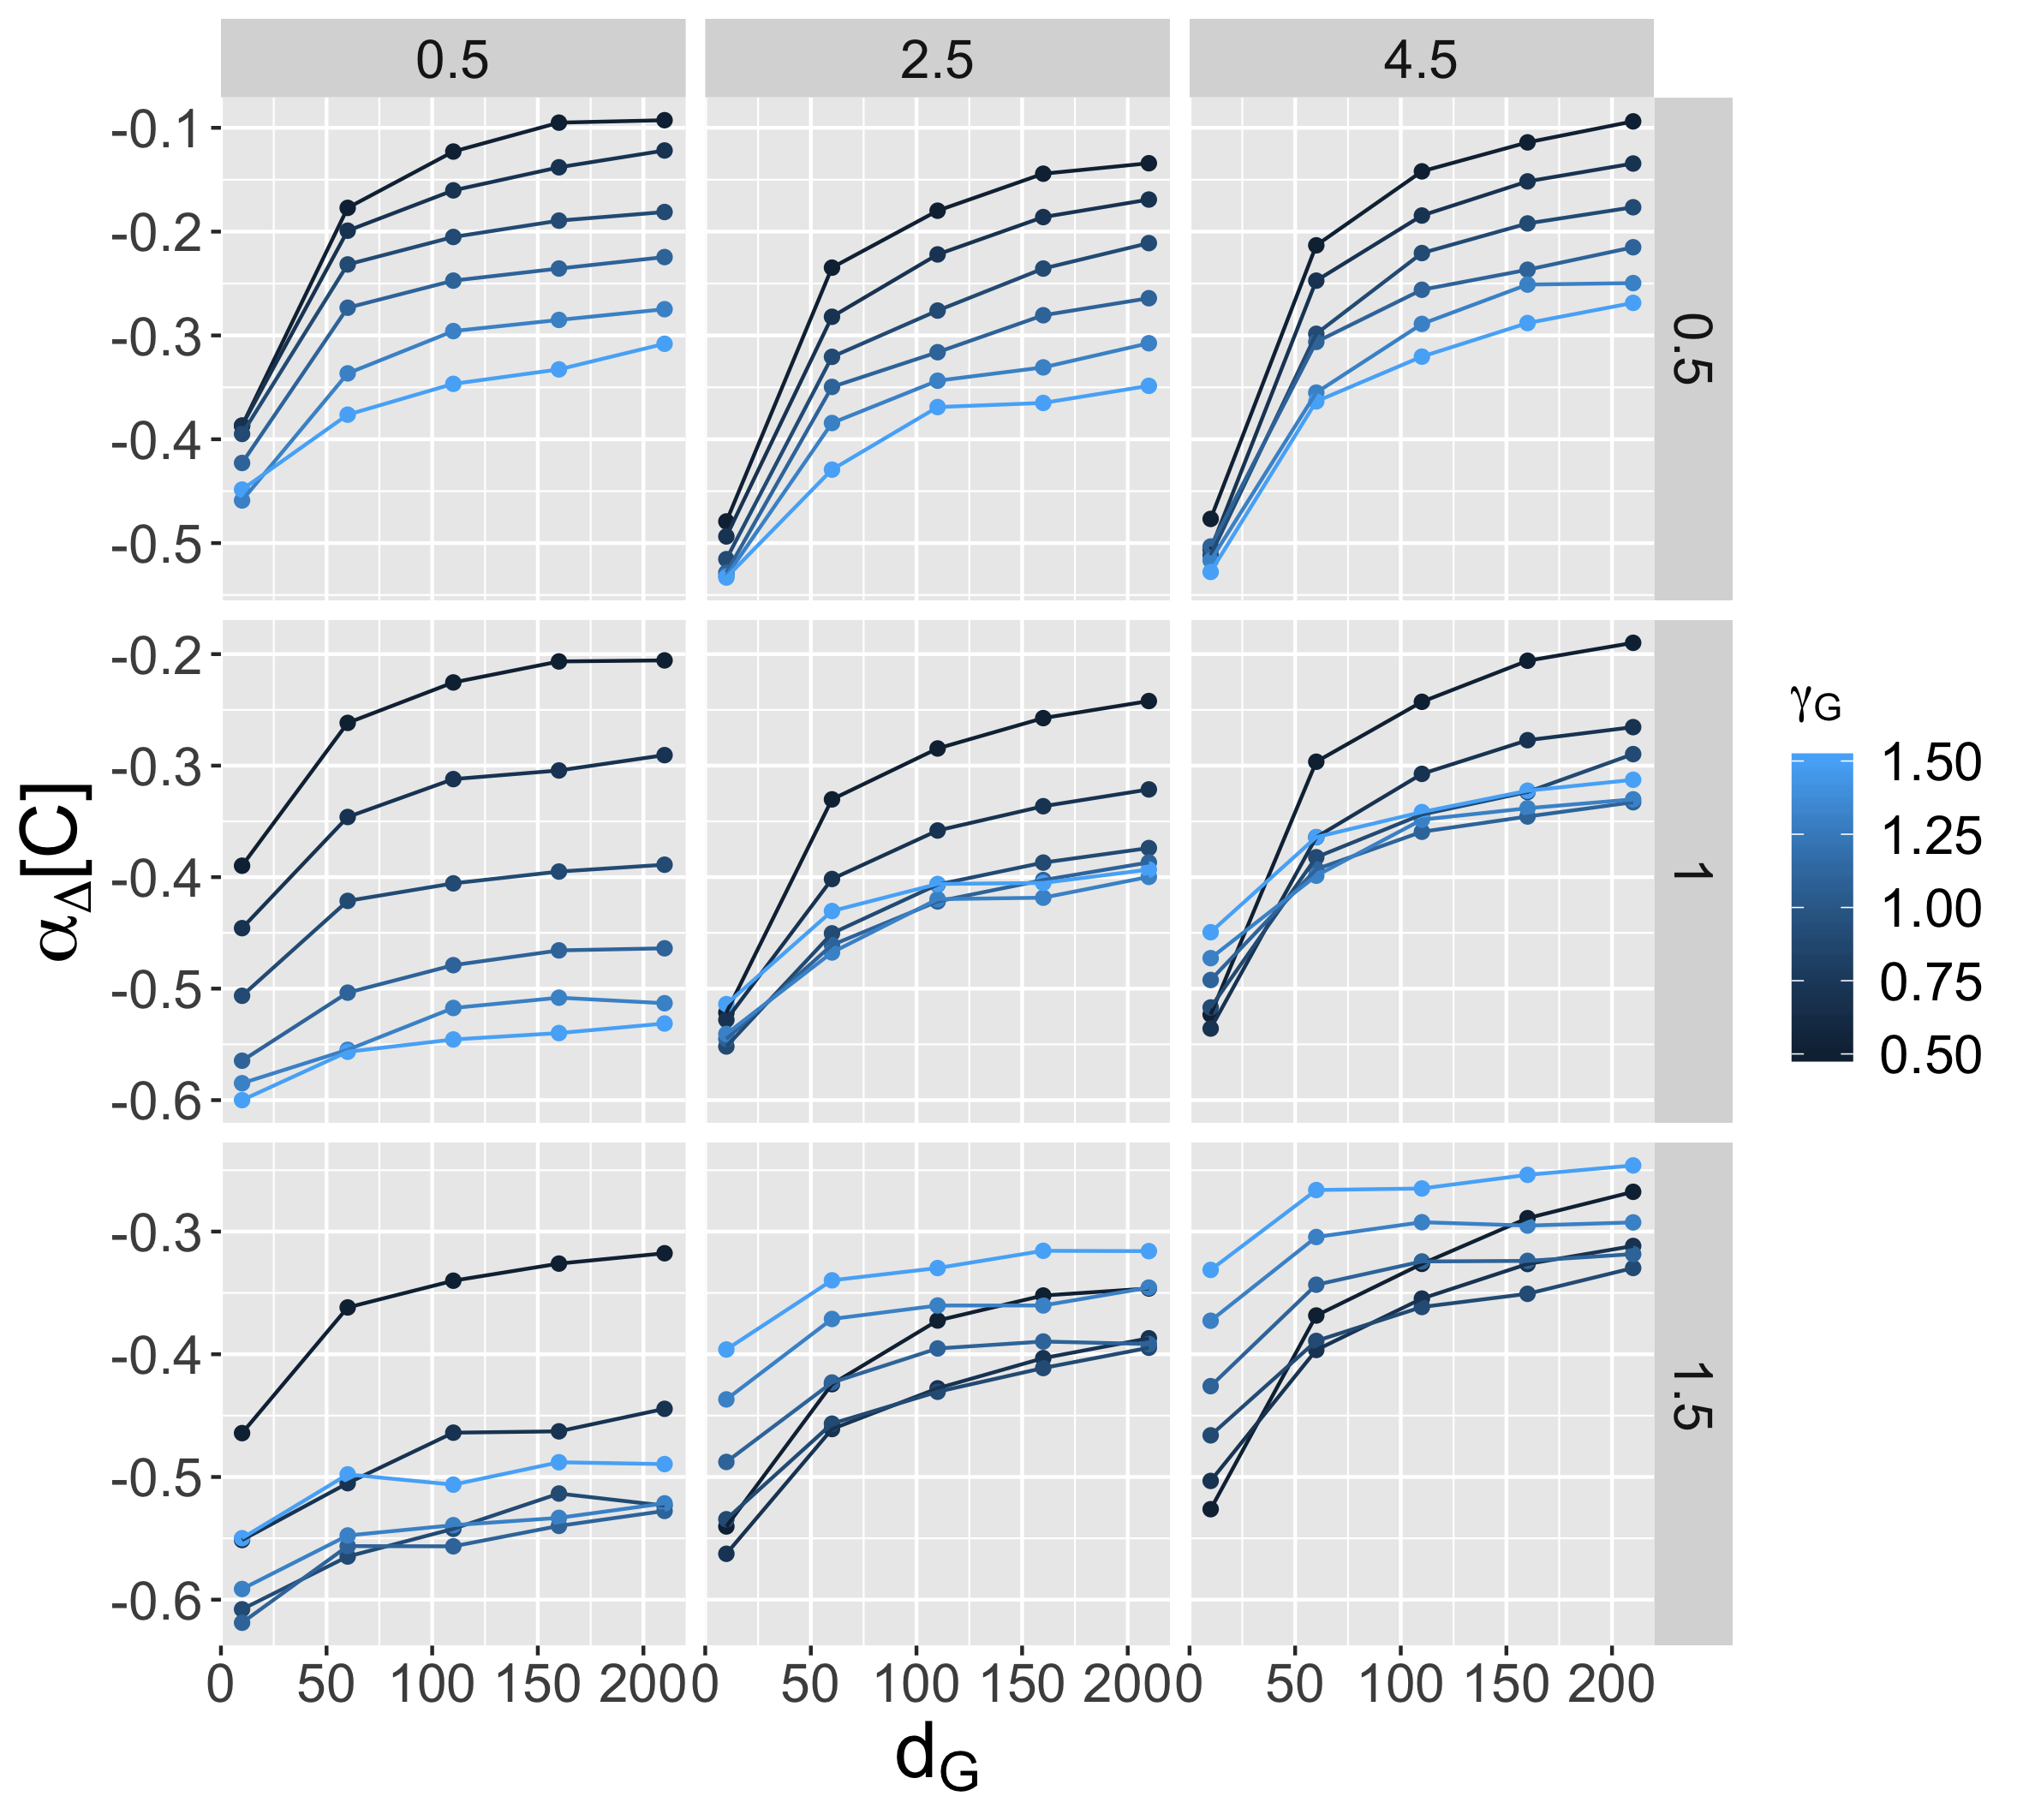
\includegraphics[width=0.48\linewidth]{figures/hierarchiesClosenessAlpha_nwExp1_wG0_001_xgravityDecay_colgravityGamma_facetsynthRankSize-nwThreshold.png}\\
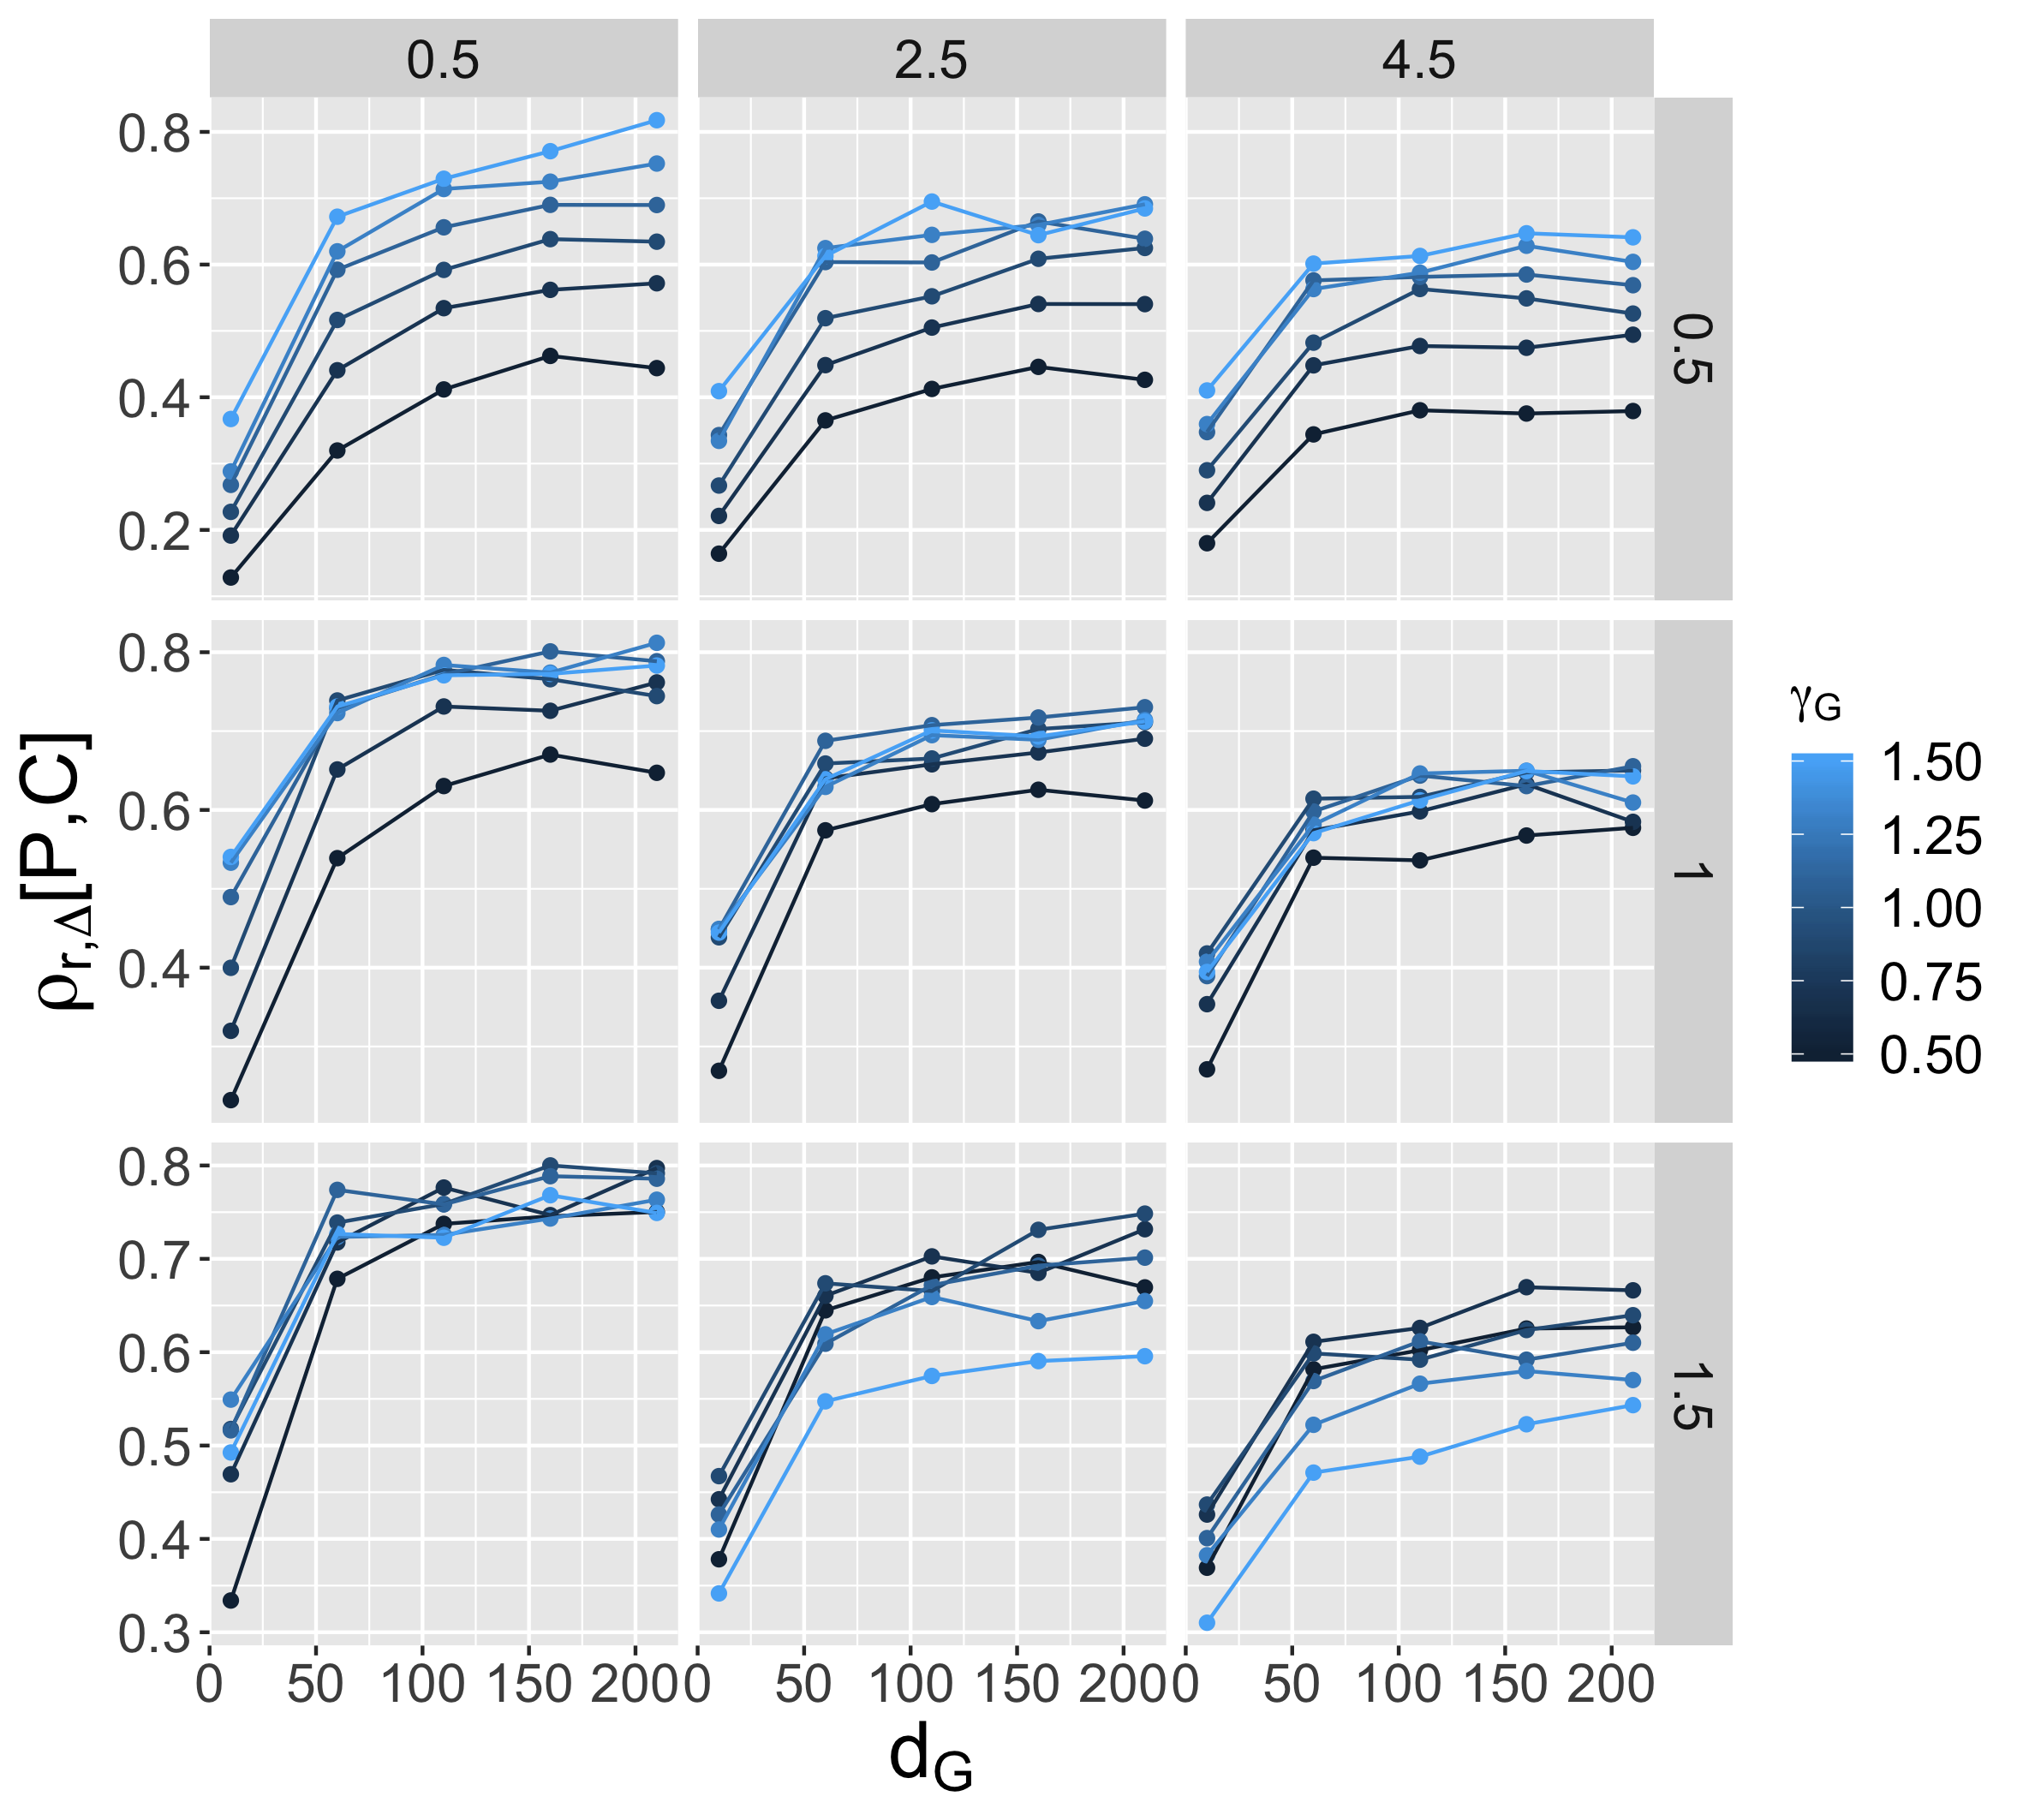
\includegraphics[width=0.48\linewidth]{figures/rankCorrsPopCloseness_nwExp1_wG0_001_xgravityDecay_colgravityGamma_facetsynthRankSize-nwThreshold.png}
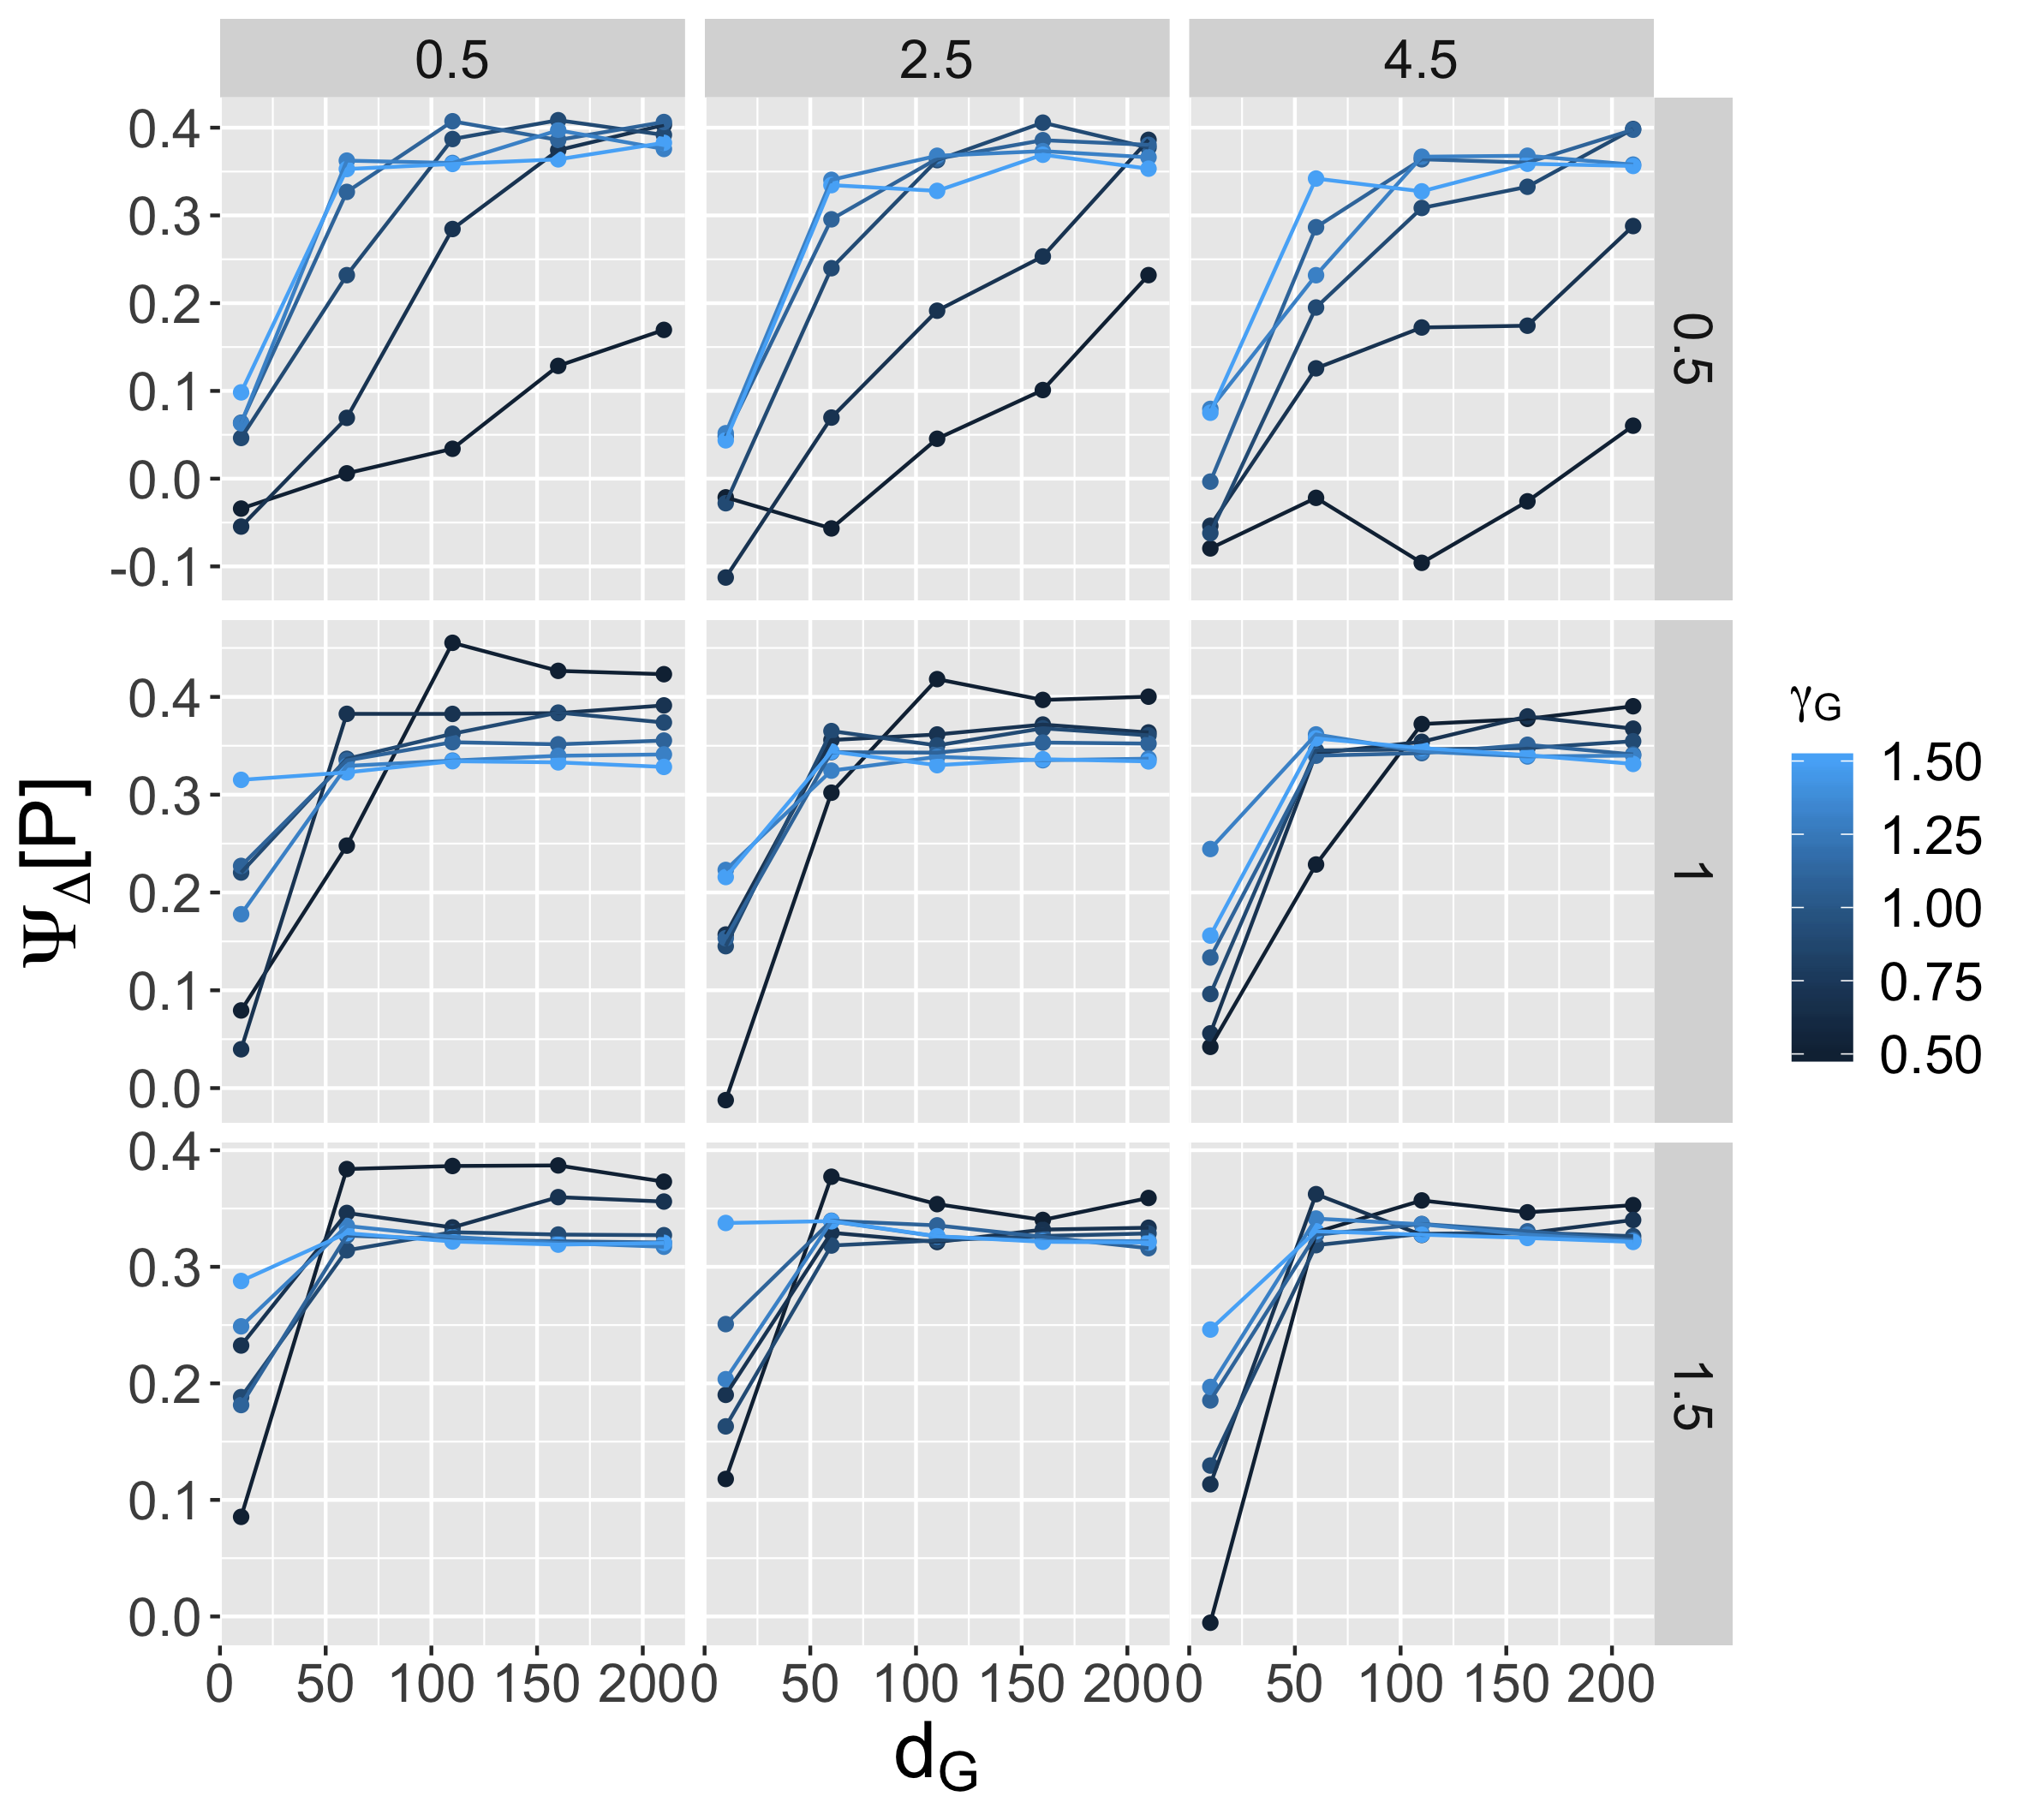
\includegraphics[width=0.48\linewidth]{figures/segHierarchiesPopPsi_nwExp1_wG0_001_xgravityDecay_colgravityGamma_facetsynthRankSize-nwThreshold.png}
\caption{\textbf{Patterns of hierarchy in the model with a virtual network.} \textit{(Top Left)} Difference in the rank-size exponent between final time and initial time, }
\end{figure}
%%%%%%%%%%%%%%

%%%%%%%%%%%%%%
\begin{figure}
\centering
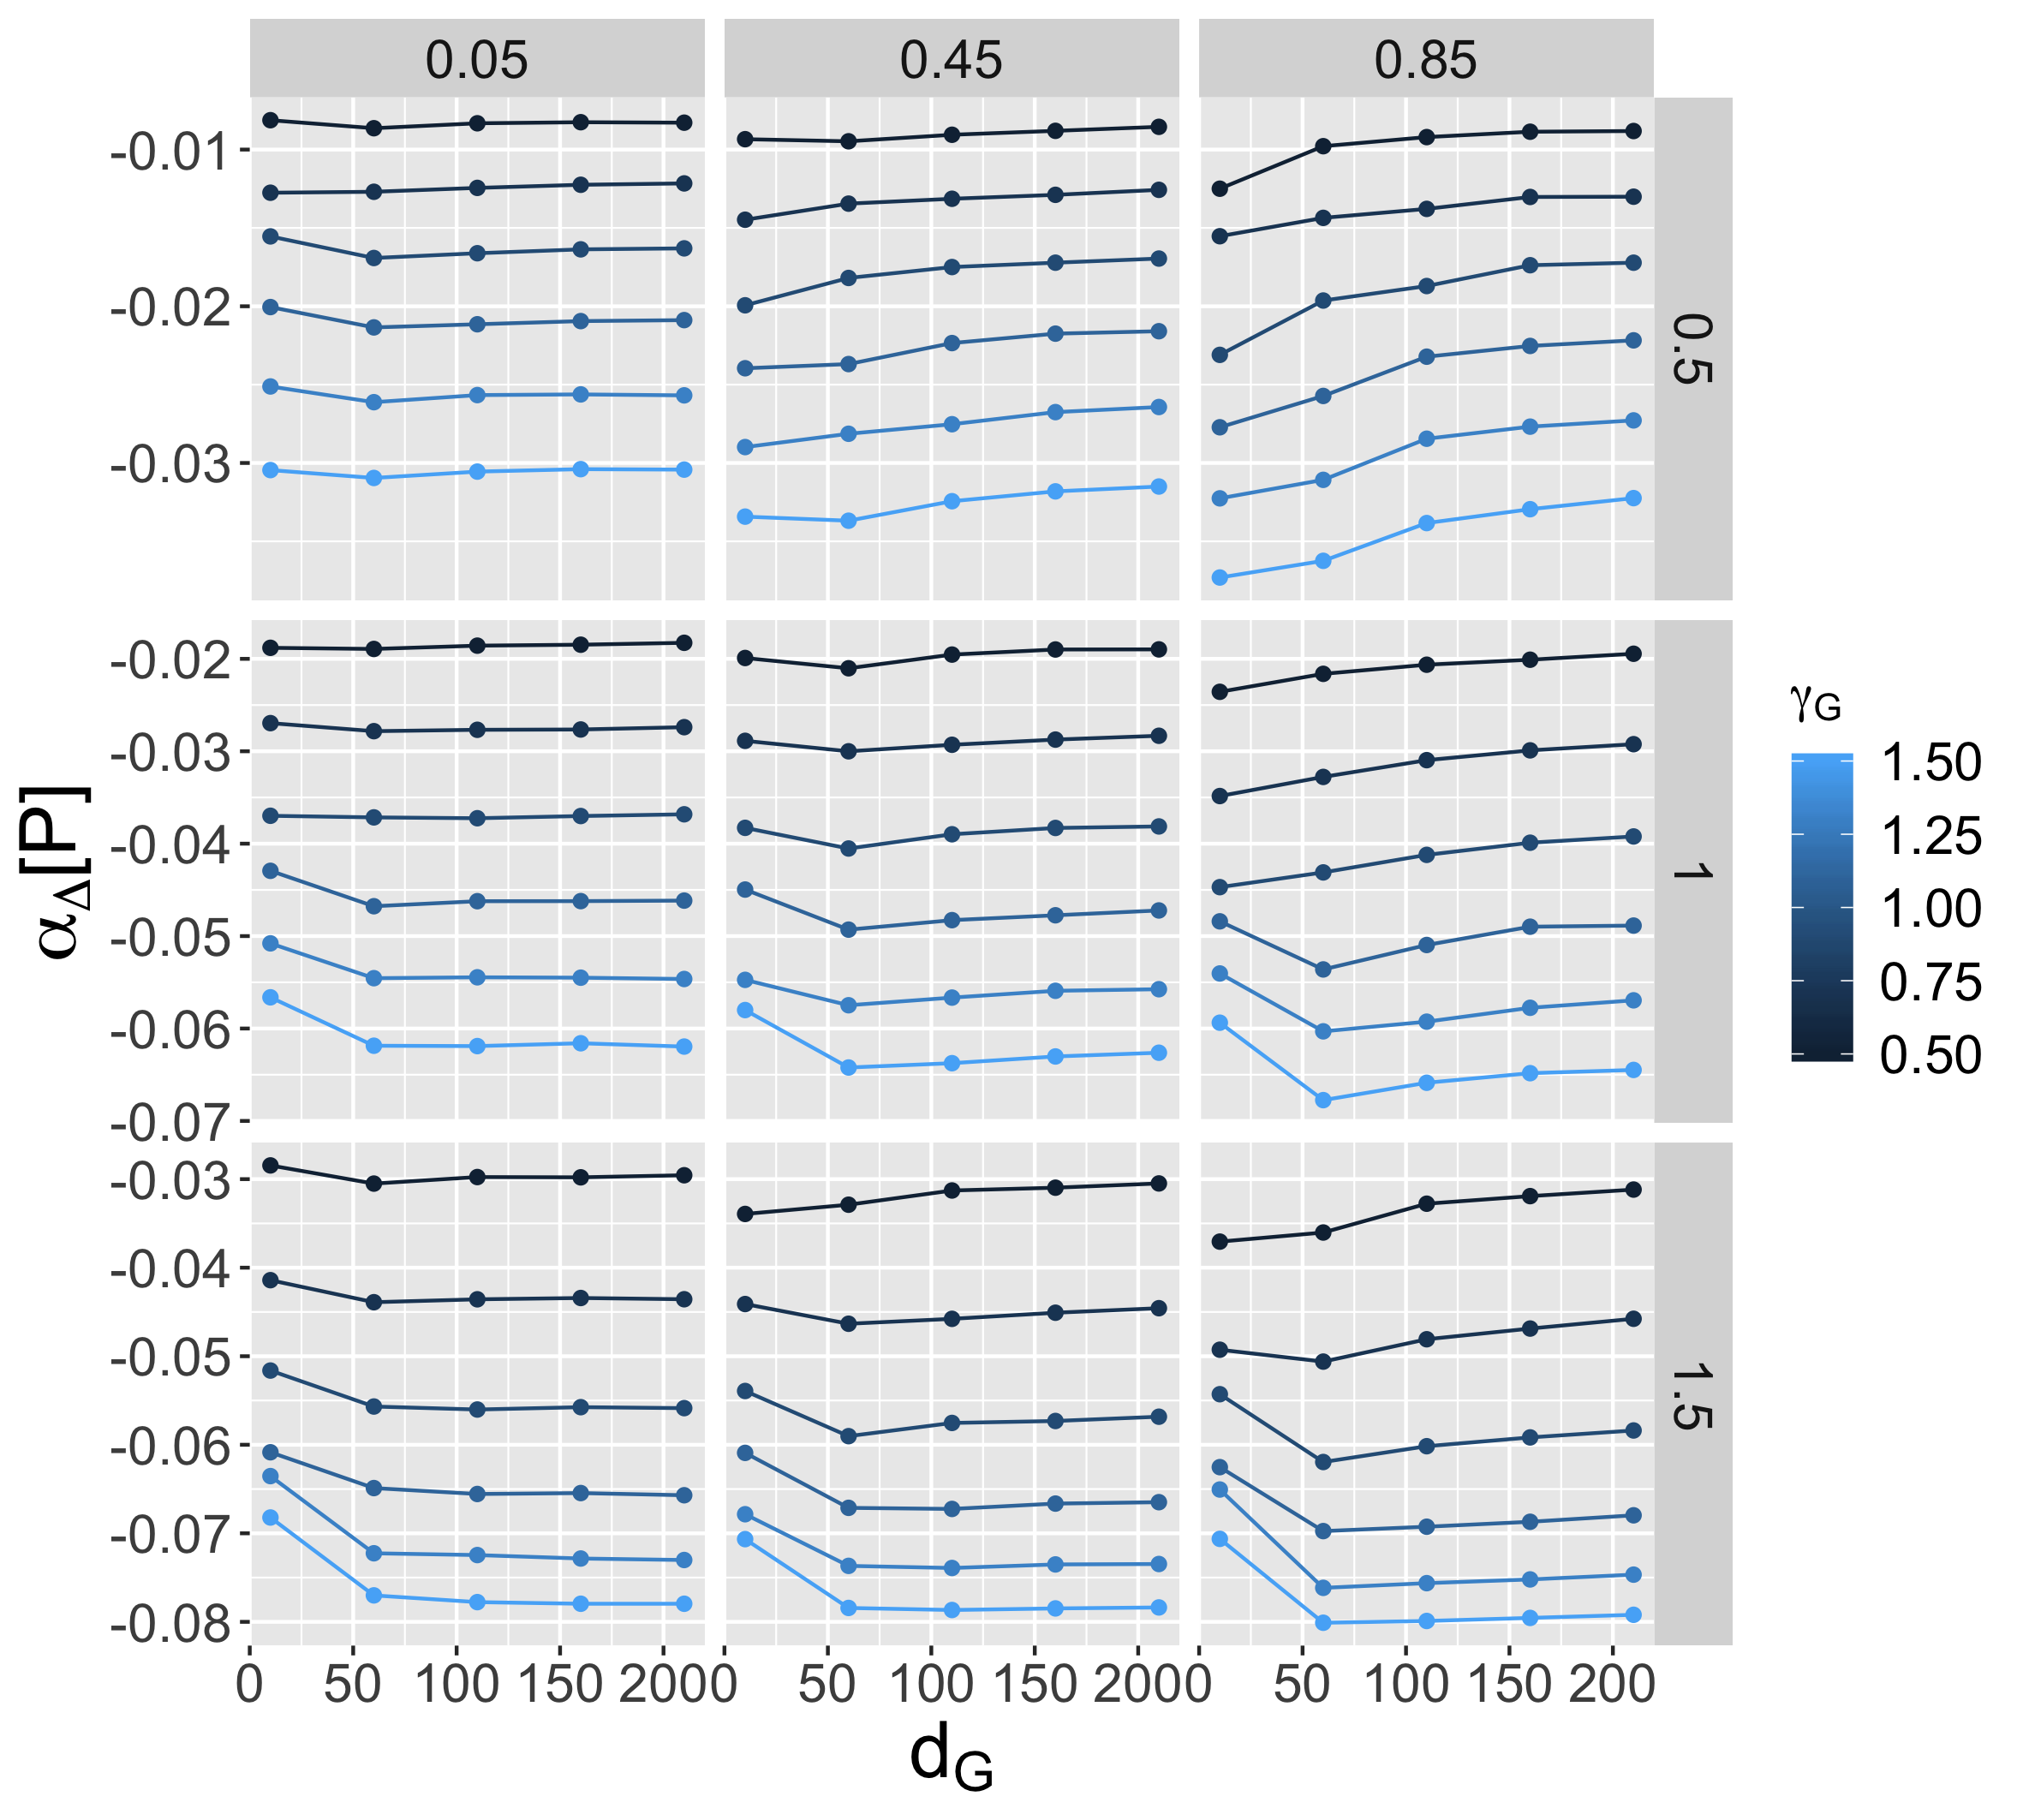
\includegraphics[width=0.48\linewidth]{figures/hierarchiesPopAlpha_nwExp1_wG0_001_xgravityDecay_colgravityGamma_facetsynthRankSize-nwPhysQuantile.png}
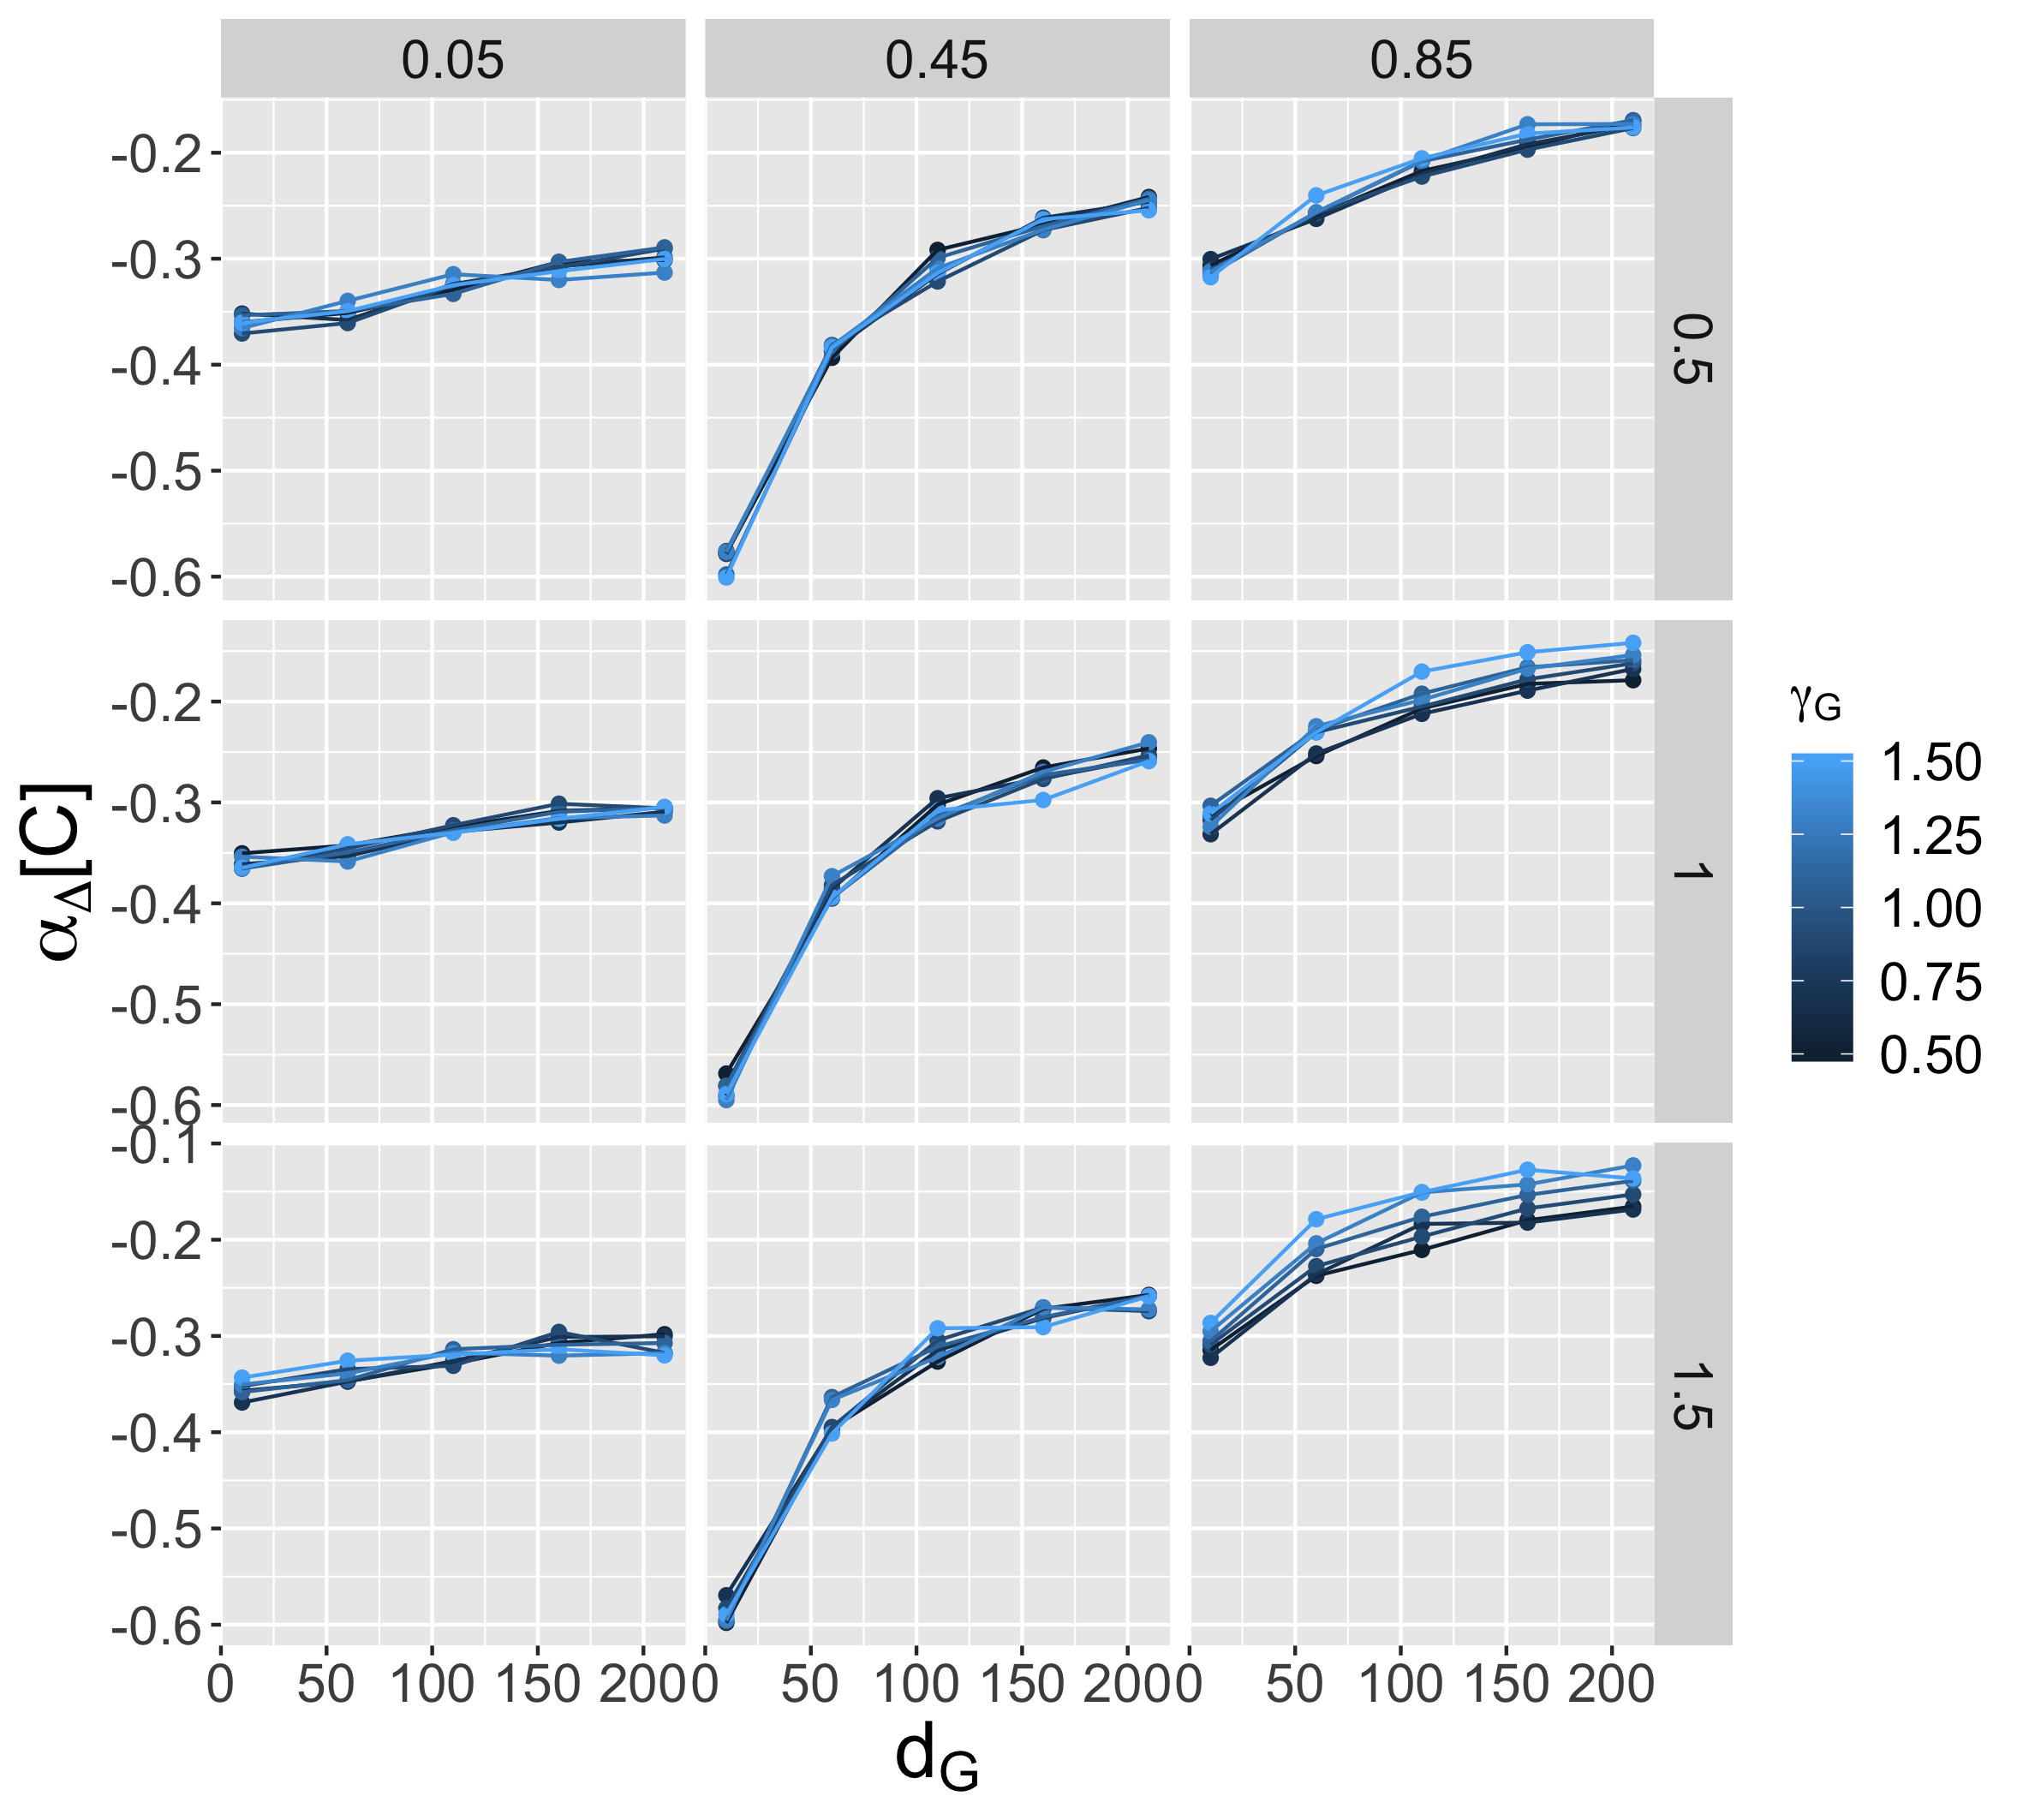
\includegraphics[width=0.48\linewidth]{figures/hierarchiesClosenessAlpha_nwExp1_wG0_001_xgravityDecay_colgravityGamma_facetsynthRankSize-nwPhysQuantile.png}\\
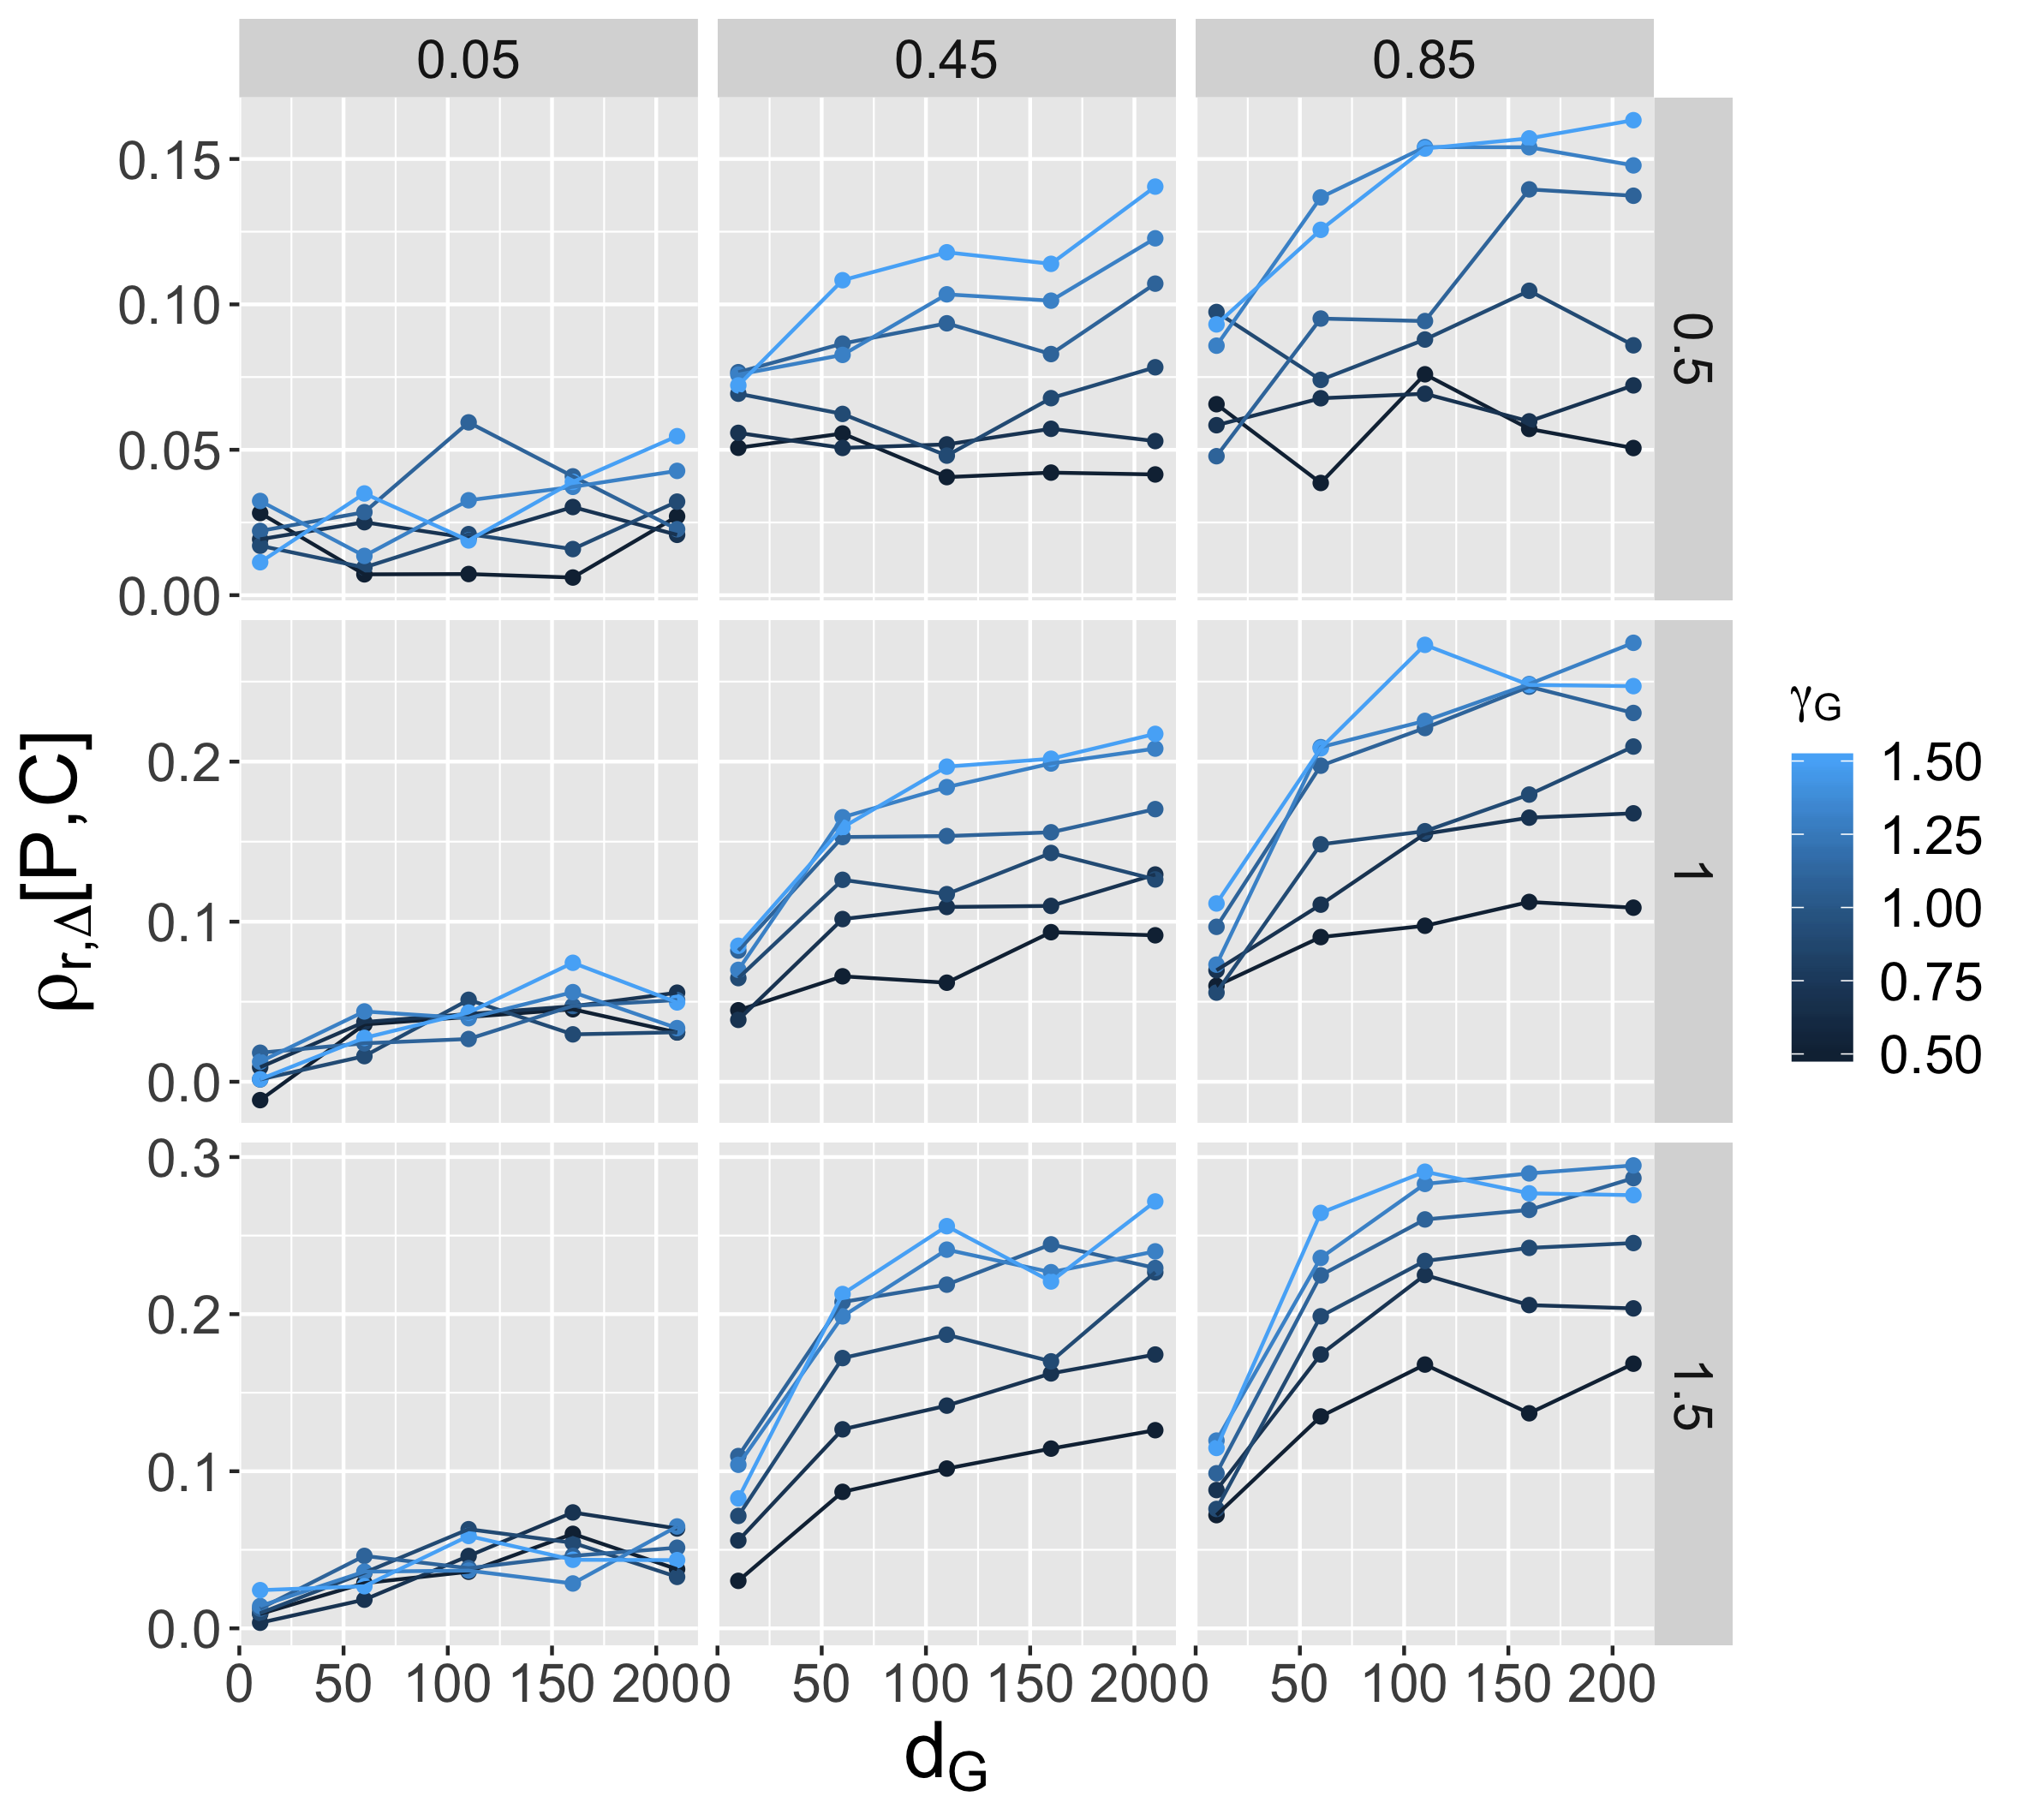
\includegraphics[width=0.48\linewidth]{figures/rankCorrsPopCloseness_nwExp1_wG0_001_xgravityDecay_colgravityGamma_facetsynthRankSize-nwPhysQuantile.png}
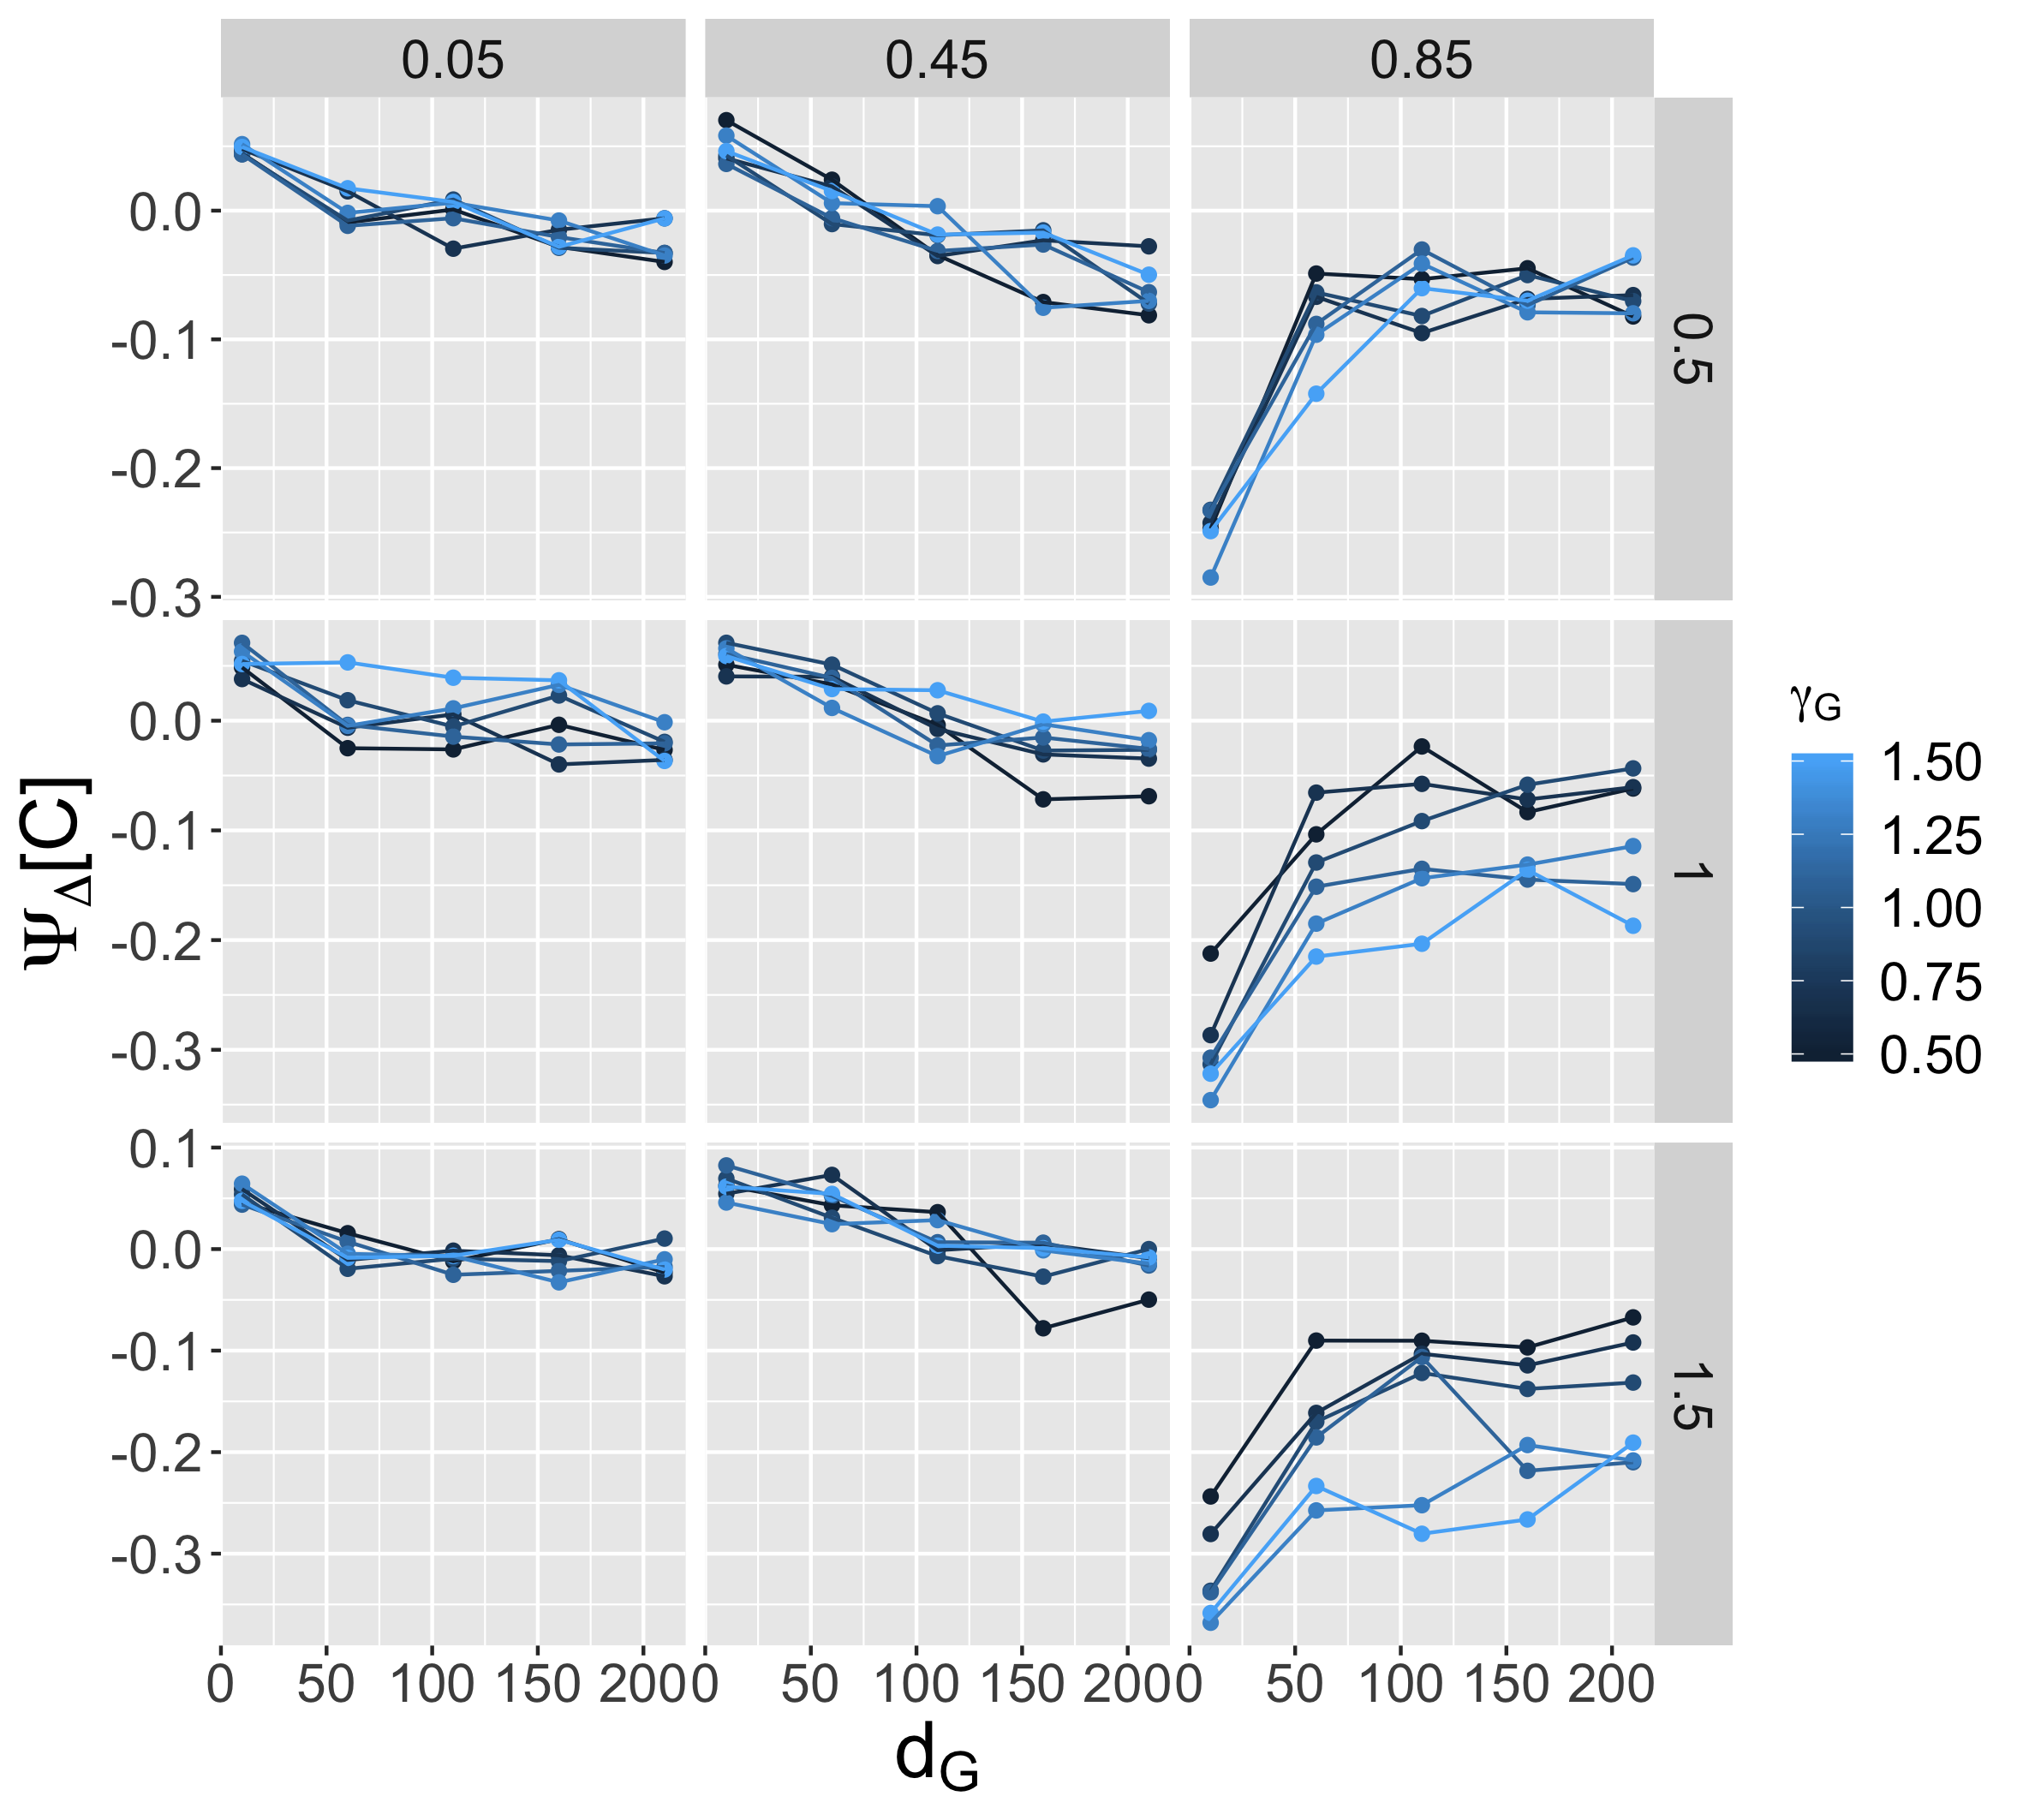
\includegraphics[width=0.48\linewidth]{figures/segHierarchiesClosenessPsi_nwExp1_wG0_001_xgravityDecay_colgravityGamma_facetsynthRankSize-nwPhysQuantile.png}
\caption{\textbf{Patterns of hierarchy in the model with a physical network.} \textit{(Top Left)}  }
\end{figure}
%%%%%%%%%%%%%%









\subsection{Hierarchy regimes}

% - PSE targeted on different regimes (dynamical ?) of hierarchy => piecewise linear fitting? 
% => simple three dimensional pattern: alpha_P, alpha_C, rho_r [P, C]








%%%%%%%%%%%%%%%%
\section{Discussion}



\subsection{Results on co-evolution and hierarchies}

% what do we learn in this particular context ?
% - teachings on the role of self-reinforcement

% the model add no links! -> in a way very similar to Levinson? - other scale and other purpose / measures



\subsection{Developments}

%\subsection{Spatial hierarchical niches}
% possible experiment: optim algo to isolate optimal fitting niches; find typical niche size when varying parameters
% (out of the scope / development of algo in itself)


\subsection{Theoretical perspective}

% ~ disc from jig ?

% \textbf{Proposition : } \textit{les hiérarchies, au sens d'imbrication de sous-systèmes à de multiples niveaux, sont endogènes aux systèmes complexes}
% des structures ``hiérarchiques'' au sens commun (structure de dépendance rigide et arborescente) sont simples et ni adaptatives ni résilientes
% le concept de hiérarchie ne peut être considéré comme exogène et totalement déconstruit
% pour l'aide à la décision, des utopies réductionnistes en horizontalité complète s'opposent aux théories de la complexité
% question ouverte (reflexive): endogènes \textit{aux systèmes} ou aux \textit{théories et modèles des systèmes} ?
%\textbf{Des approches multi-scalaires intégratives pour des gouvernances territoriales soutenables \cite{rozenblat2018conclusion} doivent prendre en compte la complexités des hiérarchies.}





%%%%%%%%%%%%%%%%
\section{Conclusion}




\bibliographystyle{agsm}
\bibliography{biblio}
%\def\pagesname{pp.~}
%\def\numbername{no.~}
%\def\pagename{p.~}



%\appendix
%\chapter{Appendix}



%\vfill\pagebreak
%\
%\thispagestyle{empty}


\end{document} 


%%%%%
%% Template 

%\begin{figure}[ptbh]
%\centering
%\includegraphics[width=10.6009cm,height=4.714cm]{GadalaExp.eps}\caption{Start and stop shear flow experiment;\break the torque would be proportional
%to the shear stress, after\break Gadala-Maria and Acrivos \cite{Gadala80}}
%\label{Fig 1}
%\end{figure}\pagebreak




